%% LyX 2.2.2 created this file.  For more info, see http://www.lyx.org/.
%% Do not edit unless you really know what you are doing.
\documentclass[English]{article}
\usepackage{mathpazo}
\renewcommand{\sfdefault}{Times}
\usepackage[T1]{fontenc}
\usepackage[latin9]{inputenc}
\usepackage{geometry}
\geometry{verbose,lmargin=3cm,rmargin=3cm}
\usepackage{babel}
\usepackage{amsmath}
\usepackage{amsthm}
\usepackage{amssymb}
\usepackage{graphicx}
\usepackage{subfig}
\usepackage{caption}
\usepackage{float}
\usepackage{multirow}
\usepackage{chngcntr}
\usepackage{array}
\usepackage{adjustbox}
\usepackage{rotating}
\usepackage{booktabs}
\usepackage{amssymb}
\usepackage[authoryear]{natbib}
\usepackage[unicode=true,pdfusetitle,
 bookmarks=true,bookmarksnumbered=false,bookmarksopen=false,
 breaklinks=false,pdfboder={0 0 1},backref=false,colorlinks=true, citecolor=blue]
 {hyperref}
\usepackage{breakurl}
\renewcommand{\baselinestretch}{1.5}
\begin{document}
\title{\Large{}A Cost-benefit Analysis of R\&D and Patents:
\\ Firm-level Evidence from China\footnote{I am grateful to Mark Roberts and Jonathan Eaton for their guidance and support throughout this project. I thank Paul Grieco and Daniel Grodzicki for their comments at the early stage of this project. I thank Jie Zhang, Fuxin, and Wenping Zheng for sharing me with the Chinese patents data. All remaining errors are mine. }}
\author{Zhiyuan Chen\footnote{Department of Economics, Pennsylvania State University. Email: chenzhiyuan1224@gmail.com.}}
\maketitle
\begin{abstract}
Building on a standard dynamic model of endogenous productivity change, I develop a flexible empirical framework to analyze the components of the returns to R\&D and quantify the patent value. Applying it to a sample of Chinese high-tech manufacturing firms, I quantify the short-run and long-run benefits of R\&D investment. I find that around 70\% of the benefits of R\&D investment comes from non-patenting innovation. On average an invention (a utility model) patent causes 0.76 (0.67) percent increase in the firm value. The start-up costs of R\&D is estimated to be around ten times as large as the maintenance costs. The counterfactual analysis shows that financing start-up innovation is more effective than financing the maintenance costs in stimulating the R\&D investment. 

\textsl{Keywords:} dynamic R\&D investment; patenting; productivity; R\&D subsidy
\end{abstract}

\newpage

\section{Introduction}

Innovation is a key engine of economic growth. Quantifying the costs and benefits of innovation activities is essential to the understanding of firm's incentives to innovate. Considering the innovation as a process of producing knowledge, R\&D is the input while patenting is part of the output. This is formally analyzed in the econometric models linking innovation outcome to R\&D investment, and allowing the productivity to be affected by the innovation output \citep{crepon1998research,mairesse2005,raymond2015}. In these models, all of the return to R\&D is captured by the innovation output which are usually measured by patents. However, since only part of the invention is patentable, these studies may obtain a biased estimate for the returns to either R\&D or patents. Moreover, only including R\&D investment in the productivity process gives no room for analyzing the structure of R\&D benefits.

Instead of viewing patents as the only innovation output, this study admits patenting as a part of innovation outcome and allows for non-patenting inventions to affect the firm's future productivity. In particular, I treat R\&D as the fundamental source of endogenous productivity growth, but the marginal effect of R\&D investment is affected by patenting activities. Therefore, my specification is an extension of the productivity process considered in the innovation and productivity literature.\footnote{See \cite{hall2010} and references therein for the productivity specifications used in estimating the return to R\&D.} This seemingly small change has ramifications in understanding the structure of return to R\&D investment. 

I embed the extended specification of endogenous productivity process into a standard dynamic structural model of R\&D investment.\footnote{See \citet{Awetal.2011,Doraszelski2013, Peters2017}} I develop an empirical strategy to decompose the benefits of R\&D into patenting and non-patenting outcome is provided. To the best of my knowledge, this paper provides a first decomposition of return to R\&D investment into patenting and non-patenting activities. Moreover, I have also developed an estimator to quantify the private benefits of patenting by calculating the marginal increase in the firm value caused by patenting. Different from \citet{pakes1986} in which the value of holding a patent is determined by solving an optimal stopping problem, this study measures the expected value of applying a patent while treating patenting as a stochastic outcome of R\&D investment. These methods can easily be applied to any data sets with information on R\&D, patents, and productivity.

I apply the model to a sample of China high-tech manufacturing firms.  The main findings from the structural estimates are as follows. First, on average R\&D investment causes around 0.45\% increase (or around 0.24 million USD) in the firm value. This is much lower than the estimates obtained by \citet{Peters2017} (PRVF hereafter), who find that R\&D investment increases firm value by 6.7 percent and 4.413 million Euros for the median high-tech firm in a sample of German firms. This provides an explanation for the low participation in R\&D investment in China. Second, a decomposition of the return to R\&D shows that non-patenting innovation accounts for a majority (around 77\%) of the total return to R\&D. Third, the average expected value of an invention (a utility) patent is around 0.39 (0.34) million USD when measured by the increase in firm value. Lastly, the start-up costs of R\&D is over ten times larger than maintenance costs. This reflects that starting a new innovation project requires a larger amount of investment than maintaining an ongoing research project. The R\&D costs distribution differs by different industries. 


I also perform a series of counterfactual exercises to evaluate the effectiveness of different types of R\&D subsidy policies that reduce the costs of R\&D investment. Some interesting results are found. First, lump-sum subsidy is universally more effective than marginal subsidy either in increasing the firm value or promoting the innovation participation. Second, for both types of the subsidy programs, reductions in the maintenance costs cause a greater increase in the firm value. But subsidizing the start-up (maintenance) costs promotes innovation participation more under lump-sum (proportional) subsidy. Third, lump-sum subsidy is more efficient than proportional subsidy. In the experiment of 20\% decrease in maintenance costs for R\&D, the average efficiency of lump-sum subsidy is around 12 times greater than the marginal subsidy in increasing firm value, and is about twice greater in promoting the firm's innovation participation. The difference is more striking when I consider the subsidy for start-up costs of R\&D. 

This study is closely related to literature on quantifying the return to R\&D. The knowledge capital model of \citet{griliches1979issues} has been a corner stone of this literature. In this framework, the investment in innovation by the firm creates knowledge stock, which is similar to physical capital in the way that they enter into the production function. The most important extension related to this paper is the econometric framework proposed by \citet*{crepon1998research} (CDM hereafter) which estimates a reduced-form model incorporates R\&D, patents, and productivity. Recently, \citet*{raymond2015} have extended this  framework to a dynamic setting. However, the knowledge-stock approach faces the problem of estimating the firm's knowledge stock. It also rules out the high degree of intrinsic  uncertainty facing innovation investment. 

Building on the knowledge capital investment model by \cite{hall1989research} and \cite{klette1996r}, the endogenous productivity approach  models the uncertainty facing the R\&D investment as assumes the productivity is unknown to the econometrician \citep{Awetal.2011, Doraszelski2013, Peters2017}. In particular, the firm's productivity is modeled as a controlled Markov process. Current R\&D investment shifts the conditional mean of the future productivity. By loading the impact of distant past R\&D expenditures in current productivity, this approach avoids
the problem of calculating the knowledge stock for each firm. With the exogenous shocks, this framework allows for different productivity levels even for firms with identical historical path of R\&D expenditures. Recently, PRVF explicitly consider the uncertainty to the innovation process and assume that only the realized innovation affects future productivity. Note that a large part of the innovation output is the accumulation of tacit knowledge that are difficult to measure. In this case, the stochastic error term in the productivity process will contain the information of R\&D investment that is positively correlated with the variables of innovation output. This endogeneity issue causes a bias to the estimates of the returns to R\&D. This paper proposes a method of dealing with this problem by allowing both the R\&D investment and innovation output enters the productivity process. 

This study contributes to the existing literature in several aspects. First, it enriches the literature on quantifying the returns to R\&D by providing a decomposition of the benefits of R\&D into patenting and non-patenting channels. The empirical finding suggests that non-patenting R\&D investment plays a major role in the returns to R\&D. Second, I provide a new method of quantifying the private value of patents. Third, the empirical implementation in this paper provides a first structural analysis on the costs-benefits structure of R\&D and patents in China, thus contributing to the literature on understanding the innovation activities in China.\footnote{See, for example, \citet{Hu2009, hu2017china,chen2017}} The estimation results show that non-patenting innovation accounts for most of the returns to R\&D. Moreover, the relative small benefits of R\&D activities and relatively high start-up R\&D costs help explain low participation in investing R\&D. 

The rest of this paper is organized as follows. In Section 2, I introduce the R\&D model and methodology for estimating the benefits of R\&D and patent value. Data are introduced in Section 3. Section 4 provides the empirical results.  Section 5 is the counterfactual analysis on the effectiveness of R\&D subsidies. Section 6 concludes the paper. 

\section{A Flexible Empirical Framework}\label{Sec2}
In this section, I first briefly lay out a standard model of dynamic model with R\&D investment and patents. The basic structure of the model is similar to that considered in \cite{Awetal.2011,Doraszelski2013,Peters2016, Peters2017}, with the exception that both R\&D and patents play a role in shifting the future productivity. 

\subsection{A Model of R\&D Investment}

\paragraph{Production and Profits} A firm has a Cobb-Douglas production function
\begin{equation}
Q_{it} = \Phi_{it}K_{it}^{\beta_{k}}L_{it}^{\beta_l}M_{it}^{\beta_m}\exp{(\beta_a a_{it})}
\end{equation}
where $Q_{it}$ is the physical output of firm $i$ in period t, $\Phi_{it}$ is the total factor productivity, $K_{it}$ is the capital, $L_{it}$ is the labor, $M_{it}$ is the material, $a_{it}$ is the firm's age. Consider a well-behaved inverse demand equation
\begin{equation}
    p_{it} = D(Q_{it})
\end{equation}
where $p_{it}$ is the output price. To simplify the analysis, we assume that a firm treats capital and productivity as predetermined when choosing labor and materials in each period. Let $\Pi(\phi_{it},\mathbf{S}_{it})$ be the optimal profits, and $R(\phi_{it},\mathbf{S}_{it})$ be the revenue, where $\phi_{it}=\ln(\Phi_{it})$, $\mathbf{S}_{it}=(K_{it}, P_{Lit}, P_{Mit}, a_{it})$ is a vector of exogenous state variables. The cost minimization implies that
\begin{equation}
    \Pi(\phi_{it},\mathbf{S}_{it}) = (1-\frac{\beta_l+\beta_m}{\theta_{it}})R(\phi_{it},\mathbf{S}_{it})
\end{equation}
where $\theta_{it}$ is the markup. Note that when $\beta_l+\beta_m=1$, the production function is of constant return to scale in terms of $L_{it}$ and $M_{it}$.

\paragraph{Productivity evolution}The firm's productivity $\phi_{it}$ is unobserved by the econometrician. R\&D investment and patenting enter the Markov process governing the productivity evolution. In particular, the dynamics of the productivity is given by
\begin{equation}
    \phi_{it+1} = h(\phi_{it},d_{it},\mathbf{o}_{it+1})+\epsilon_{it+1}
\end{equation}
where $d_{it}$ represents the R\&D investment and $\mathbf{o}_{it+1}$ is a vector summarizing the innovation outcome next period, and $\epsilon_{it+1}$ is an iid shock with a mean-zero normal distribution. Considering different types of innovation output, $\mathbf{o}_{it}$ can be a vector of process innovation and product innovation measured by the patents or other observed indicators. The marginal effects of R\&D investment and innovation output are captured by three partial derivatives $\partial h/\partial d_{it}$, $\partial h/\partial \mathbf{o}_{it+1}$, and a cross derivative $\partial ^2h/\partial d_{it} \partial \mathbf{o}_{it+1}$. Because R\&D is the fundamental source of productivity change, we impose that $ \partial h(\phi_{it}, 0, \mathbf{o}_{it+1})/\partial\mathbf{o}_{it+1} = \mathbf{0}$. This implies that without R\&D investment, we should expect no endogenous productivity growth, though we can see productivity growth through the channel of exogenous shocks. The cross-derivative $\partial ^2h/\partial d_{it} \partial \mathbf{o}_{it+1}$ deserves some discussion. When positive, it means that the stimulating impact of R\&D on productivity is strengthened through the patenting. This indicates that the patenting system help firms protect their inventions. When negative, we anticipate that the effect of knowledge spillovers dominates so that firms productivity improves less by patenting. This may be due to the weak patenting system.

Following CDM, I assume that patents is a random variable of which the distribution is determined by R\&D investment. This assumption greatly simplifies the analysis by only considering the R\&D investment choice. Specifically, patents outcome in next period is assumed to be a distribution depending on past R\&D. The distribution of $\mathbf{o}_{it+1}$ is given by $Pr(\mathbf{o}_{it}\leq \mathbf{o}) = G(\mathbf{o};d_{it})$.\footnote{In the reduce-form analysis, this process is usually estimated using count data models. See \cite{hall1989research,hall2010}.} This layer of uncertainty is similar to that considered in PRVF. Note the Markovian property implies that the conditional expectation of future productivity is 
\begin{equation*}
    \mathbf{E}(\phi_{it+1}|\phi_{it}, d_{it})=\int h(\phi_{it},d_{it},\mathbf{o})dG(\mathbf{o};d_{it})
\end{equation*}
Therefore R\&D investment can influence future productivity through affecting $h(\phi_{it}, d_{it},\mathbf{o})$ and the distribution of innovation output $G(\mathbf{o}; d_{it})$. This allows me to decompose the impact of R\&D into patenting and non-patenting channels.


\paragraph{Recursive formulation}
To consider a general setting, denote $C(d_{it}, \mathbf{X}_{it})$ as the variable costs of R\&D investment. Here $\mathbf{X}_{it}=(\mathbf{S}_{it}, \mathbf{Z}_{it})$, $\mathbf{Z}_{it}$ is the additional exogenous states that influence the costs of R\&D investment.\footnote{For example, $\mathbf{Z}_{it}$ may contain past R\&D investment decisions so the R\&D costs also include adjustment costs.} In addition, there is a fixed cost of R\&D investment, denoted as $f(\mathbf{X}_{it})$. With this fixed costs, the model can capture the innovation choice at the extensive margin. Note that we allow the exogenous state variables to affect the costs of R\&D. Omitting the subscripts, the firm's dynamic programming problem can be written in a recursive formulation:
\begin{equation}\label{VF_full}
    V(\phi, \mathbf{X}) =\max_{d}\left\{V^0(\phi, \mathbf{X}), V^d(\phi, \mathbf{X})\right\} 
\end{equation}
where the value functions for different choices of $d$ are
\begin{align}
    V^0(\phi)&=\Pi(\phi,\mathbf{X})+ \beta \mathbf{E}\left[ V(\phi', \mathbf{X}')|d=0\right], \\
    V^d(\phi)&=\max_{d} \left\{ \Pi(\phi,\mathbf{X})-C(d, \mathbf{X}) - f(\mathbf{X}) + \beta \mathbf{E}\left[ V(\phi', \mathbf{X}')|d\right]\right\}, \label{VF_d}
\end{align}
where $\beta$ is the discounting factor. We assume that firms have perfect foresight for the exogenous state variables. This allows us to calculate the expected firm value as
\begin{equation}\label{EV_d}
    \mathbf{E}\left[ V(\phi', \mathbf{X}')|d\right] = \int\int V(h(\phi,d,\mathbf{o})+\epsilon,\mathbf{X}')dG(\mathbf{o};d)dF(\epsilon)
\end{equation}
where $F(\cdot)$ is the distribution of $\epsilon'$. 
A stochastic equilibrium of the model is a decision rule $d(\phi, \mathbf{X})\geq0$ such that the recursive problem (\ref{VF_full}) is solved.
\subsection{Benefits of R\&D and Patent Value}
\paragraph{Decomposition of the returns of R\&D} 
Following PRVF, I define the long-run benefits of R\&D investment as relative change in the expected firm value caused by R\&D investment. One novelty in this paper is that I decompose the R\&D benefits into patenting and non-patenting channels. For what follows, I use the notation of partial derivatives by assuming that both $d$ and $d$ and $\mathbf{o}$ are continuous variables and we consider the continuous region in the value function to simplify the notation. Using (\ref{EV_d}), I decompose the benefit of innovation as:
\begin{align}  \label{LB}
    LB(\phi,\mathbf{X})& = \frac{\partial \ln[\mathbf{E}(V(\phi',\mathbf{X}')|d)]}{\partial d} \\
                       & = \frac{1}{\mathbf{E}[V(\phi',\mathbf{X}')|d]} \int \left\{ \int \frac{\partial V(h+\epsilon,\mathbf{X}')}{\partial d}dG(\mathbf{o};d) + \int V(h+\epsilon,\mathbf{X}')dg(\mathbf{o};d) \right \}dF(\epsilon) \nonumber
\end{align}
where $g(o;d_{it})$ is the density function. This provides a decomposition of firm value change into two channels. The first term on in the big bracket captures the direct impact of R\&D on future firm value, which is the non-patenting channel. R\&D investment also influences the distribution of innovation outcome, this impact is captured in the second term. Notice that in models with only R\&D investment enters the productivity evolution (like \citet{Doraszelski2013}), only the first term appears. In the model where only innovation outcome matters for productivity (such as \citet{Peters2017}), only the second term shows up. Specification (\ref{LB}) nests them as special cases. As a result, the benefits of innovation can be viewed as a composition of two parts:
\begin{align}
    LB_{N}(\phi,\mathbf{X})&= \frac{1}{\mathbf{E}[V(\phi',\mathbf{X}')|d]} \int\int \frac{\partial V(h+\epsilon,\mathbf{X}')}{\partial d}dG(\mathbf{o};d)dF(\epsilon), \\
    LB_{P}(\phi, \mathbf{X})&=   \frac{1}{\mathbf{E} [V(\phi',\mathbf{X}')|d]}\int\int V(h+\epsilon,\mathbf{X}')dg(\mathbf{o};d)dF(\epsilon), \label{LB_P}
\end{align}
where $LB_{N}$ is the part of R\&D returns without patenting, $LB_{P}$ represents the portion of the benefits of R\&D realized through patenting. Though we use patents as an example here, this decomposition strategy can also be directly applied to models in which innovation input and output differs. The underlying assumption in my model is conditional on the observed innovation output, R\&D still plays a role in affecting the firm performance.
\paragraph{Patent value}
To obtain the value of patents, we need to fix the firm's R\&D investment so that the benefits of R\&D is not confounded with the value of patents in determining the firm value. We then compute the increase change in the firm value by exogenously adjusting the value of innovation output. Let $\mathbf{E}[V(\phi',\mathbf{X}')|d,\mathbf{o'}]$ be the expected firm value conditional on R\&D investment and innovation output, we obtain that
\begin{equation}\label{EV_do}
    \mathbf{E}[V(\phi',\mathbf{X}')|d,\mathbf{o'}] = \int V(h(\phi,d,\mathbf{o}'),\mathbf{X}')dF(\epsilon)
\end{equation}
Note that we remove the uncertainty in generating innovation output by conditioning on $\mathbf{o'}$. Then we differentiate the log-form of (\ref{EV_do}) with respect to $\mathbf{o}'$ and obtain an estimator for the patent value:
\begin{align}
    PV(\mathbf{o}', d) &=  \frac{\partial \ln [\mathbf{E}(V(\phi',\mathbf{X}'|d,\mathbf{o}')]}{\partial \mathbf{o'}} \\
                     &=  \frac{1}{\mathbf{E} [V(\phi',\mathbf{X}')|d, \mathbf{o}']} \int\frac{\partial V(h(\phi,d,\mathbf{o}')+\epsilon,\mathbf{X}')}{\partial \mathbf{o}'}dF(\epsilon) \nonumber
\end{align}
Notice $PV(\mathbf{o}',d)$ has a dimension identical to $\mathbf{o}'$. Let $o_{j}$ be the $j^{th}$ element in $\mathbf{o}$. We call $o_j$ as the outcome of $j$-type innovation. Also let's denote $\mathbf{o}_{-j}$ as a vector of elements in $\mathbf{o}$ excluding $o_j$. In particular, if $\mathbf{o}\in \mathbf{R}^n$, $\mathbf{o}_{-j}=(o_1,\cdots,o_{j-1},o_{j+1},\cdots,o_n)$. In principle, there are interacting effects among different elements in $\mathbf{o}'$. That is, the value of $j$-type innovation $PV_j(\mathbf{o}',d)$ varies by $\mathbf{o}'_{-j}$. To avoid this complication, we compute the average value of each type of patent by using the distribution of $\mathbf{o}'_{-j}$ conditional on $j$-type innovation and R\&D investment $d$. Given the joint distribution $G(\mathbf{o}';d)$, the conditional distribution $G(\mathbf{o}_{-j}'|o_j',d)$ is given by
\begin{equation*}
    G(\mathbf{o}'_{-j}|o_j',d) =\int \frac{g(\mathbf{o}';d)}{g_j(o_j';d)}d\mathbf{o}_{-j}'
\end{equation*} 
where $g_j(o_j;d)=\int g(\mathbf{o}';d)d\mathbf{o}_{-j}'$ is the the marginal density function of $o_j$. Employing this probability distribution, we define the value of $j$-type innovation output as
\begin{align}
    EPV_j(o_j,d) = \int PV(\mathbf{o}',d)dG(\mathbf{o}'_{-j}|o_j,d).
\end{align}
Notice that the calculation of $EPV_j$ does not depend on the realizations of $\mathbf{o}'_{-j}$. The conditional expectation also characterizes the linkages between different types of innovation output. 
\paragraph{Extensive margin of R\&D} R\&D data often contains measurement error, and patent data are count data. This encourages researchers to  This situation can easily be accommodated by the empirical framework in this paper. Now we consider the R\&D choice $d\in\{0,1\}$ and patent count data $o_j\in\mathbb{N}$. We only need to slightly change the notation. First, the R\&D benefits is defined only at the extensive margin:
\begin{equation}
    DLB(\phi,\mathbf{X}) =\ln\mathbf{E}[V(\phi',\mathbf{X}')|d=1]-\ln\mathbf{E}[V(\phi',\mathbf{X}')|d=0]
\end{equation}
Using a similar decomposition, the non-patenting and patenting benefits are:
\begin{align}
    DLB_N(\phi,\mathbf{X}) =& G(\mathbf{0};d=1)\left\{\int \ln V(h(\phi,d=1,\mathbf{0}),\mathbf{X}')dF(\epsilon)-\ln\mathbf{E}[V(\phi',\mathbf{X}')|d=0]\right\} \label{DLB_N} \\ 
    DLB_P(\phi,\mathbf{X}) =&\int \int_{\mathbf{o}>\mathbf{0}}\left\{\ln V(h(\phi,d=1,\mathbf{0}),\mathbf{X}')-\ln\mathbf{E}[V(\phi',\mathbf{X}')|d=0]\right\}dG(\mathbf{o};d=0)dF(\epsilon) \label{DLB_P}
\end{align}
where $G(\mathbf{0};d=1)$ is the probability that no patent generated and $\mathbf{o}>\mathbf{0}$ means that each element in $\mathbf{o}$ is strictly positive. These two expressions are simply a discrete version of the decomposition introduced before. To consider the patent value, we can define the value of $j$-type innovation output as 
\begin{equation} \label{patent_value}
    DEPV_j(o_j,d) = \int PV(\mathbf{o}',d=1)dG(\mathbf{o}'_{-j}|o_j,d=1)-\int PV(\mathbf{o}',d=1)dG(\mathbf{o}'_{-j}|o_j-1,d=1)
\end{equation}
Note $G(\mathbf{o}'_{-j}|o_j-1,d=1)$ captures the probabilistic distribution of all types when no $j$-type patent is generated. Once again, the patent value is defined as the marginal change in the expected firm value generated by increasing the number $j$-type patent by one. 

\section{Application}
In this section, I employ the introduced empirical framework to provide a quantitative analysis of the benefits of R\&D and patents. I first introduce the data source. Based on the data features, I adapt the general empirical framework to quantify the two main components of R\&D benefits as well as the patent value. 

\subsection{Data}
\subsubsection{Data sources}
\paragraph{Firm-level production data}
The first data set contains information on the large and medium sized Chinese manufacturing firms from 2001 to 2007 complied by China's National Bureau of Statistics (CNBS
hereafter). This data set is widely used in studies on Chinese firms (See \citet{HsiehKlenow}, \citet*{song2011}, and \citet*{BRANDT2012339} for example).
This data set includes all Chinese State Owned Enterprises (SOEs hereafter)
and non-SOEs with annual sales no less than five million \textit{Renminbi}
(equivalent to about 700,000 US dollars). These firms accounts for
98\% of the manufacturing exports. This data set contains all the
information of the firm's major accounting sheets, which includes
more than 100 financial variables. Serving for the purpose of this study, it includes firm
sales, number of employees, material input, fixed assets, R\&D expenditures,
and firm characteristics like firm age and its industrial code. In
summary, this rich data set provide the information on the firm-level
production activities. I have obtained a sample of high-tech manufacturing firms from this dataset. 
\paragraph{Patent data}
The second database it on patent statistics collected by the State
Intellectual Property Office (henceforth SIPO) of China. It contains
all the patents that are applied by Chinese firms and certified in mainland China. For each patent the database has the information on its type (invention, utility model, and design), owner, application
time, certification time, agent of application, abstract, location,
and expiration time during 1985 and 2012. But it should be noted that
there is no information on citations for patents in the database,
which makes it difficult to measure the patents quality directly. According to China's Patent Law, the utility model refers to a new technical solution suitable for practical use proposed for the shape, construction or combination of the products. Generally, an invention patent is also related to a new technical solution proposed for the product, method or its improvement. But the patenting process for invention patent consists of a "substantive review" which specifically emphasizes on the novelty and originality of the breakthrough in technical upgrading. Obviously, lower creativity standards are enforced for utility model patents. Invention patents, however, may be of less practicability and generate less profits. As for design patents, they represent more rudimentary type of innovation and are considered to be of lower quality than invention patents and utility model patents (\citet{hu2017china}).\footnote{ According to Article 22 of the Patent Law of the P.R.C.: any invention
or utility model for which patent right may be granted must possess
novelty, inventiveness and practical applicability. In comparison,
the requirement for the approving of design patents is in Article
24 of the Patent Law of the P.R.C as \textquotedblleft \dots \dots must
not be identical with or similar to any design which, before the date
of filing, has been publicly disclosed in publications in the country
or abroad or has been publicly used in the country, and must not collide
with any legal prior rights obtained by any other person.\textquotedblright{}}
 Therefore we anticipate that design patents is less related to firm's productivity. Considering this, I will focus on invention patents and utility patents in the empirical investigation. 

\paragraph{Final combined database}

For the purpose of this study, I merge these two data sets using the
firm name. Table \ref{T1} shows aggregate information on the number of patents
for the combined database. The aggregate number of invention patents
and utility patents show a strong increasing trend over the sample
period. One important concern on using the combined data set is the
efficiency of matching between these two data sets. To evaluate the
matching efficiency, in the last row of Table \ref{T1}, I show the percentage
of the total number of invention patents in the merged data set to
the figure published in the China Statistical Yearbook on Science
and Technology. We find that this ratio varies across years, with
55.57\% in 2007 and 96.35\% in 2003. Overall, the merged dataset captures most of the information in the patents data.
\begin{center}
Table \ref{T1} here
\par\end{center}

\subsubsection{Descriptive Statistics}
China's
high-tech industries mainly covers four 2-digit industries: pharmaceutical
manufacturing, special equipment, electric machinery, and electronics. In Table \ref{T2} I report the summary statistics for the R\&D and patenting activities in the final dataset. The average R\&D expenditure for high-tech manufacturing firms is
218.095 thousand yuan (equivalent to around 31,584 US dollars).
The R\&D intensity measured by total R\&D expenditures over total sales is relatively low than that reported for developed countries. Lastly, compared to the R\&D participation, we observe that the probability of generating a patent is much lower. 

\begin{center}
Table \ref{T2} here
\par\end{center}

In Figure \ref{F1}, I display the number of firms for each 2-digit high-tech industry
by their innovative activities. As shown in Figure \ref{F1}, even
for the high-tech manufacturing firms in China, only a small portion of firms
undertake R\&D investment. The fraction
of firms that file patent applications is even smaller. The difference
between R\&D activities and patent applications imply that distinguishing
the input of innovation and output of innovation is important when
thinking of the costs and benefits of innovation because R\&D activities with patents may generate larger impact on the firm's productivity. The decline in the number of firms also suggests that innovative firms face uncertainty in generating patents. 

\begin{center}
Figure \ref{F1} here
\end{center}

I also notice that in the data, the extensive margins of R\&D and patents capture a majority of the innovation activity. These data features are presented in the data appendix. Moreover, \citet*{mairesse2005} provide evidence on the substantial measurement error of using R\&D expenditure to predict the innovation probability for the firm-level data from the French innovation survey. Also \citet*{chen2017} also document that corporate income tax reductions induce Chinese firms to relabel administrative expenses as expenditures on R\&D. These results suggest that the levels of R\&D may not accurately reflect the firm's actual investment in innovation. Therefore using discrete R\&D choice as a measure of R\&D investment can also help decrease measurement error.

\subsection{Empirical Model and Estimation Results}
Given the data features, I outline an empirical model to analyze the returns to R\&D and patenting. This model is a variant of the empirical framework introduced in Section \ref{Sec2}, thus providing an application of the empirical framework to a particular dataset from China. To some extent, the empirical model resembles the structural model by PRVF. The difference is I focus on the decomposition of R\&D benefits. To simplify the notation, I will omit time and firm subscripts whenever no confusion arises. Moreover, $Z'$ represent the next-period $\mathbf{Z}$, and $z=ln(Z)$
\subsubsection{Productivity Estimation}
I assume that the demand is CES with elasticity of $\sigma$: $Q_{it}=P_{it}^{-\sigma}P_t^{\sigma}Q_t$, where $P_t$ and $Q_t$ are the sectoral price index and output, respectively. We consider the case that $\beta_l+\beta_m=1$.\footnote{It is had to separately identify $(\beta_l+\beta_m)$ separately from $\sigma$ without information on the output prices.} It can be shown that the log of short-run revenue is:
\begin{equation}\label{log-rev}
    r(\phi_{it}, \mathbf{S}_{it}) =\mu_{0}+\mu_{t}+(\sigma-1)(\beta_kk_{it}+\beta_a a_{it}+\phi_{it})
\end{equation}
where$\mu_0$ is the constant and $\mu_t$ is a year-specific variable common to all firms.\footnote{See math appendix for the algebra.} In principle, $\phi_{it}$ contains the idiosyncratic shifter in the demand. The short-run profits is a constant fraction of the revenue:
\begin{equation}
    \Pi(\phi_{it},\mathbf{S}_{it})=\frac{1}{\sigma}\exp(r(\phi_{it},\mathbf{S}_{it}))
\end{equation}
In light of the discussion above, we use 0-1 binary variables to measure the R\&D activities, invention patents applications, and utility patents applications. Specifically, we use $d$, $n$, and $b$ to represent the investment in R\&D, application of invention
patents, and application of utility patents. $d$ is equal to one
when the firm invests in R\&D; similar definitions are applied to
$n$ and $b$. By these notations, the innovation outcome variable $\mathbf{o}=(n,b)$. I parameterize the productivity process as a cubic function of lagged productivity:
\begin{align} \label{mk}
\phi_{it+1} =& \rho_{0}+\rho_{1}\phi_{it}+\rho_{2}\phi_{it}^{2}+\rho_{3}\phi_{it}^{3} \\
             & +\rho_{4}d_{it}+\rho_{5}\left(n_{it+1}\times d_{it} \right)+\rho_{6}\left(b_{it+1}\times d_{it}\right)+\varepsilon_{it+1} \nonumber 
\end{align}
where the first line on the right-hand side captures the persistence
of productivity, the second line describes the impacts of R\&D and
patents on the evolution of productivity. It is clear that the effect
of past R\&D activity on current future productivity is affected by
the creation of new ideas. We expect
that $\rho_{5}$ and $\rho_{6}$ are different from each other because
different types of patents represent different forms of realized innovation. To a large extent, the invention patents are more related to product innovation, while
the utility patents are more related to process innovation. These
parameters give us information on the quality of patents (or ideas) to some extend.
For example, when $\rho_{5}>\rho_{6}$, invention patents have a larger impact on enhancing the productivity.

I follow \citet{Doraszelski2013} to estimate the productivity using the first-order condition of materials.The demand for materials is dependent on the observed capital stock, age, and unobserved productivity. This gives us an expression for the productivity:
\begin{equation}
\phi_{it-1}=\left(\frac{1}{1-\sigma}\right)\beta_{t-1}+\beta_{k}k_{it-1}+\beta_{a}a_{it-1}-\frac{1}{1-\sigma}m_{it-1}\label{productivity}
\end{equation}
where $\beta_{t}$ represents the the intercept of the demand function
and the variable input prices. Combining (\ref{productivity}) and (\ref{mk}) and plugging them into (\ref{log-rev}) yields an empirical equation for
the firm revenue:
\begin{align} \label{nls}
r_{it}=& \left(1-\sigma\right)\beta_{k}k_{it}+\left(1-\sigma\right)\beta_{a}a_{it}-\rho_{1}\left[\beta_{t-1}+\beta_{k}\left(1-\sigma\right)k_{it-1}+\beta_{a}\left(1-\sigma\right)a_{it-1}-m_{it-1}\right] \\
 & -\frac{\rho_{2}}{1-\sigma}\left[\beta_{t-1}+\beta_{k}\left(1-\sigma\right)k_{it-1}+\beta_{a}\left(1-\sigma\right)a_{it-1}-m_{it-1}\right]^{2} \nonumber \\
 & -\frac{\rho_{3}}{\left(1-\sigma\right)^{2}}\left[\beta_{t-1}+\beta_{k}\left(1-\sigma\right)k_{it-1}+\beta_{a}\left(1-\sigma\right)a_{it-1}-m_{it-1}\right]^{3} \nonumber \\
 & -\left(1-\sigma\right)\left[\rho_{4}d_{it-1}+\rho_{5}\left( n_{it}\times d_{it-1}\right)+\rho_{6}\left( b_{it} \times d_{it-1}\right)\right]+ \mu_{0}+\mu_{t}+v_{it} \nonumber 
\end{align}
where $v_{it}=u_{it}-\left(1-\sigma\right)\varepsilon_{it}$ and 
$u_{it}$ is the measurement error to the revenue and exogenous to
the firm's decision s on choosing variable inputs or investment in
R\&D. The estimation of (\ref{nls}) relies on the condition that
the composite error $v_{it}$ is uncorrelated with all the explanatory
variables on the right-hand side. $\mu_{0}$ is an intercept which
combines constants from the revenue function and the productivity
process. $\mu_{t}$ and $\beta_{t-1}$ are functions of the common
time-varying variables including the demand intercept and factor prices. The higher-order powers on $\phi_{it-1}$ enables us to distinguish
$\beta_{t-1}$ from $\psi_{t}$ and identify up to a base-year normalization. Following in PRVF, I use the Non-Linear Least Square estimator to estimate
the revenue equation. To account for the differences in the revenue functions
and the demand elasticity, $\mu_{0}$ is interacted with industry
dummies. Once I obtain the estimates
of $\beta_{t-1}$, $\beta_{k}$, $\beta_{a}$, I can recover the productivity
using Equation (\ref{productivity}). Then $\rho_{0}$ can be estimated
using the mean zero moment condition for $\varepsilon_{it}$. We employ a two-step estimation strategy. In the first step, we estimate the demand elasticity. In the second step, we replace $\sigma$ with its estimates and employ NLLS estimator for \ref{nls}.

For each industry, note that the ratio of total
variable costs to firm revenue $VC/R$ is equivalent to $\left(1-1/\sigma \right)$.
Therefore, for industry $j$, we can estimate $\sigma$ by using the
average of the ratio of variable costs to revenue:
\begin{equation}
\hat{\sigma}_{j}=-\frac{\sum_{it}R_{it}}{\sum_{it}(VC_{it}-R_{it})}
\end{equation}
Table \ref{T11} reports the estimation results. Notice that $\sigma$
varies across industries. For the electronics industry, the estimate of
$\sigma$ is $6.34$, the corresponding markup is 1.187. In comparison,
for the machinery industry, the demand elasticity is estimated
to be $-5.043$, implying the a markup of 1.247. We can also find
that the estimates of $\sigma$ are smaller than that obtained by
\citet{Peters2017} using German data.
This may imply that Chinese high-tech firms have a lower markup than
Germany high-tech firms. 

\begin{center}
Table \ref{T11} here
\par\end{center}

I plug the estimates of $\sigma$ into (\ref{nls}) to estimate the
parameters for the productivity evolution equation.
Table \ref{T12} reports the full estimation results. Column (1) shows
the estimation results of including $d_{t}$, $n_{t+1} \times d_{t}$,
and $b_{t+1} \times d_{t}$ in addition to 3d order polynomials of
current productivity. The estimation results show the impact of R\&D on productivity hinges
on the patenting activities. Note that the marginal effect of $d_{t}$
on the expectation of future productivity is $\rho_{4}+\rho_{5}n_{t+1}+\rho_{6}b_{t+1}$, the estimates of which are as follows:
\[
\frac{\Delta\mathbf{E}\left(\phi_{t+1}|\phi_{t},d_{t}\right)}{\Delta d_{t}}=.00435+.0145\times n_{t+1}+.0137\times b_{t+1}
\]
This indicates that patents play an important role in enhancing the
productivity effect of R\&D. If we think of a firm with
positive investment in R\&D in current period, then the expected increase
in productivity would be $\frac{.0145}{.00435}\approx 3.33$ times
greater if it can produce an invention patent in future period and
$\frac{.0137}{.00435}\approx 3.15$ times greater if it produces an utility
patent in next period. 
\begin{center}
Table \ref{T12} here
\par\end{center}

In the model, patents are channels through which
R\&D spurs the productivity growth. This is different from the PRVF model in which the impact of R\&D on future productivity is fully captured by realized
process or product innovation. PRVF find
that the coefficient of realized process innovation is 0.029 and that
of realized product innovation is 0.036 for German high-tech firms.
Our results are smaller than these estimates if we consider invention
patents as realized product innovation while utility patents as realized
process innovation. This implies that the productivity-growth effect of realized innovation is smaller for Chinese firms. 

For the endogenous productivity approach, an implicit condition for
a firm to be active in innovative activities is that the productivity
cannot increase or decrease too fast in order for it to innovate. Otherwise, the productivity is unbounded in the future, which discourages firms from investing in R\&D. The estimation results show that the revenue productivity is between -0.454 and 0.817, which implies that the absolute value of first-order derivative of expected future productivity with respect to current productivity is less than one, thus satisfying the requirement for the value function estimation. In the appendix, I display the range of this slope. I also try a quadratic specification
in which only the first- and second-order of $\phi_{t}$ are included. However, in this case, the fraction of observations that violates this assumption is not negligible; the corresponding results are displayed in appendix \ref{appc2}.

\subsubsection{R\&D-patents relation}
 Given that innovation variables are discrete, the conditional distribution of innovation outcome can be written as:
  \begin{equation}
      G(x,y;d) = Pr(n'=x,b'=y;d)
  \end{equation}
where $x,y,d\in\{0,1\}$
  . By formulating the R\&D-patent linkage as
a conditional joint cumulative distribution function, we implicitly
take the correlation between invention patents and utility patents
into consideration. This can be caused by the
idea diffusion within the firm. We also expect that firms engaging
in R\&D activities are more likely to produce invention or utility
patents. Lastly, we do not model the possibility that different firms have different inclination to protect their ideas by creating patents. 
However, by selecting high-tech industries, we try to alleviate the concern that some firms may not want to protect their innovation via patenting because high-tech firms are more willing to file patent applications
when they create new ideas. 
In addition, our sample period starts
from 2002, before which China has implemented several amendments to
patents law aimed to strength the protection of intellectual property
rights \citep{Hu2009}. As a result, our measure is an average of the industry-specific propensity of submitting patent applications.

We estimate the probability of producing applicable patents conditional
on the firm's past R\&D status. For notation simplicity, $P\left(n_{t+1}=x,b_{t+1}=y|d\right)$
is denoted as $P\left(x,y|d\right)$. For each industry, our estimator
for the conditional probabilities is given by 
\begin{equation}
\hat{P}\left(x,y|d\right)=\frac{\sum_{i}\sum_{t}\mathbb{I}\left(n_{it+1}=x\right)\mathbb{I}\left(b_{it+1}=y\right)}{\sum_{i}\sum_{t}\mathbb{I}\left(d_{it}=d\right)}
\end{equation}
where $\mathbb{I}\left(\cdot\right)$ is the indicator function and
$x,y,d\in\left\{ 0,1\right\} $. This procedure imposes that the
probability of filing patent applications only depends on the firm's
past R\&D activity. Moreover, the technology of generating patent applications is common to all firms within the same industry. 

The results are displayed in Table \ref{T10}.
We can find that these probabilities are different in
different industries. While the pharmaceutical industry is better at producing invention patents, the other three industries create more utility model patents. This may imply that product innovation is more prevalent in pharmaceutical industry, but the process innovation is more common in other high-tech industries. Last but not the least, there is a certain probability that product innovation is discovered along with process innovation. 
\begin{center}
Table \ref{T10} here
\par\end{center}

\subsubsection{R\&D costs and benefits}
Following PRVF, the innovation cost is assumed to be dependent on prior
R\&D experience and current capital stock. The costs of R\&D investment $C$ follows an exponential distribution:
\begin{equation}
C\sim \exp \left(\kappa^m kd_{-1}+\kappa ^s k(1-d_{-1})  \right)\label{d cost}
\end{equation}
where $\exp(\cdot)$ represents the exponential distribution, $d_{-1}$ is the R\&D decision in previous period. Hence the cost of investing in R\&D follows an exponential distribution with a mean of $\kappa ^m k$ when $d_{-1}=1$, and with a mean of $\kappa ^sk$ when $d_{-1}=0$. This formulation allows that $\kappa ^m$ and $\kappa ^s$ to be different, implying that the distribution of maintenance costs and start-up costs are different. $k$ enters the distribution of R\&D costs because of the scale effect that a firm with larger capital stock are required to hire more researchers and build larger research labs; $k$ will be treated as exogenous. The realize of the cost is known to the firm, but not to the econometrician. To simplify the notation, I denote the mean of the R\&D costs distribution as $\gamma \equiv \kappa ^m d_{-1} k+\kappa ^s  (1-d_{-1})k$.
The state variables are $\mathbf{X}=(\phi, d_{-1},\mathbf{S})$. Now the firm's value function $V(\phi, d_{-1}, \mathbf{S})$ can be calculated as:

\begin{equation}\label{VF}
V(\phi, d_{-1},\mathbf{S})=\left\{ \Pi(\phi,\mathbf{S})+ \int_{0}^{\infty}\max_{d\in\{0,1\}}\left\{\beta\mathbf{E}V_{0},  \beta \mathbf{E}V_{1}-c\right\}dH(c) \right\} 
\end{equation}
where $\beta$ is the discount factor and $H(c)=1-e^{-c/\gamma}$ when $c\geq0$ and zero otherwise, and 
\begin{align}
  \mathbf{E}V_{0} &= \sum_{n'}\sum_{b'}\int_{\phi'}V(\phi',d,\mathbf{S}')dF(\phi'|\phi,n',b',d=0)G(n',b'|d=0) \label{EV0} \\
  \mathbf{E}V_{1} &=\sum_{n'}\sum_{b'}\int_{\phi'}V(\phi',d,\mathbf{S}')dF(\phi'|\phi,n',b',d=1)G(n',b'|d=1) \label{EV1}
\end{align}
The expression for $\mathbf{E}V_{1}$ is just a special case of (\ref{VF_d}). Given the innovation cost $c$, the firm will invest in R\&D if
\begin{equation}\label{Cutoff}
\Delta EV(\phi, d_{-1},\mathbf{S})\equiv \beta \mathbf{E}V_{1}-\beta \mathbf{E}V_{0}\geq c
\end{equation}
That is a firm will only invest in R\&D as long as the expected net benefit from R\&D is greater than its costs. Using (\ref{Cutoff}), we can express the firm's probability of investing in R\&D as:
\begin{align}\label{p_d}
Pr(d=1|\phi, d_{-1},\mathbf{S})=&Pr\left[\Delta EV(\phi, d_{-1},\mathbf{S})\geq c  \right] \\
                    =&1-\exp\left[-  \frac{\beta}{\gamma} ( \mathbf{E}V_{1}- \mathbf{E}V_{0}) \right] \nonumber
\end{align}
where the second equality comes from the assumption that the R\&D costs follow an exponential distribution. Knowing $(\kappa ^s, \kappa ^m)$ allows us to characterize the distribution of R\&D costs given the information on capital stock and past R\&D choice. Equation (\ref{p_d}) indicates that $\beta$ can not be separated from $\gamma$ without additional assumption. Therefore we employ the annual deposit rate to set the value for $\beta$. Let $\bar R$ be the average real annual deposit rate. The annual real deposit rate is cited from \citet{song2011} and $\bar R=1.1075$ , we choose $\beta =1/1.0175=0.983$. 

I follow \citet{Rust1987} to apply the nested fixed point algorithm to estimate the dynamic discrete choice model. To implement this algorithm, we discretize the productivity space into 100 grid points, the capital stock into 50 grid points. Remember that we have 4 categories of ages and two states for past R\&D experience. Therefore, we estimate the value function for $100\times 50 \times 4\times 2=40000$ types of firms. I use the methodology proposed by \citet{farmer2017} to discretize the non-linear Markov process specified for the productivity evolution. Finally, we assume that the costs are i.i.d across all firms and periods, then the cost parameters can be estimated using the Maximum Likelihood Estimator (MLE)  obtained by solving following problem:
\begin{equation}
\max_{(\kappa^{s},\kappa^{m})}\left\{\sum_{i}^{N}\sum_{t}^{T_i} \log \left[ d_{it}Pr(d_{it}=1|\phi_{it},d_{it-1},\mathbf{S}_{it}')+(1-d_{it})Pr(d_{it}=0|\phi_{it},d_{it-1},\mathbf{S}_{it}')\right] \right\}
\end{equation}
where $N$ is the sample size of the firm, $T_i$ is the number of periods in which firm $i$ exists in the data. The details of computation and data processing before undertaking the computation are presented in the appendix of computation.

In Panel A of Table \ref{T13}, I display the estimation results of the cost parameters $(\kappa ^s,\kappa ^m)$. In all of the four high-tech industries, we find that the start-up costs of investing in R\&D are over ten times larger than the maintenance costs. The estimates also show much differences in the maintenance costs and start-up costs for different high-tech industries. The electronics industry has the largest start-up costs and maintenance costs. This is consistent with that developing new technologies and new ideas on producing electronic products requires relatively more R\&D investment either in terms of starting R\&D activities or maintaining innovation. On the other hand, the pharmaceutical industry has the lowest start-up costs while the machinery sector has the least the maintenance costs in continuing R\&D. However, one caveat about the interpretation of the results is that our estimates of the costs have taken the government's subsidy on R\&D activities into consideration. This may bias the estimates downward, and the severity of the bias will be positively correlated to the actual amount of subsidy received by the firms in the sample.

To see these results more clearly, I also translate these estimates into average R\&D costs. The average R\&D costs is calculated by plugging the average capital stock into the equation of the mean of R\&D cost distribution. This measurement also takes the average size of firms in the industry into consideration. I report the results in Panel B of Table \ref{T13}. The average starting costs lie between .797 million US dollars for pharmaceutical industry to 2.241 million US dollars for the electronics industry. While the maintenance costs range from 87 thousands of US dollars to 143 thousands of US dollars. The difference in the magnitudes of start-up costs and maintenance costs help explain the high persistence in the R\&D investment. 
\begin{center}
Table \ref{T13} here
\end{center}
\subsubsection{Model fitness}
The model contains several pieces and are estimated in different stages. I first check the model fitness of the revenue equation by showing the closeness between the revenue predicted by our model and that in the data. In addition, the dynamic model can generate optimal R\&D choice given the firm type observed in the data. I compare the model-predicted R\&D activities with that in the data from two aspects: first, as a cross-section check, I consider the probability of investing in R\&D; second, I also check to what extent the model generated transition dynamics for R\&D fits the data. Overall, the estimated model provides a good match for these moments in the data, giving us confidence to perform further structural analysis on the benefits of R\&D and patents. The details of these checks on the model fitness are presented in the appendix.

\subsection{Benefits of R\&D investment}
\subsubsection{Aggregate results}
The short-run benefits of R\&D investment is directly reflected by the changes in productivity, which shifts sales and profits upward in subsequent periods. In comparison, the long-run gains of R\&D can be captured by the changes in the firm's expected future value.r\footnote{Note that under the CES demand structure, the proportional change in the profits is the same as that in revenue.} I also report the absolute change in firm value to evaluate the long-run benefits of R\&D more completely. Note that the measure of benefits is independent of past R\&D activities. However, past R\&D activities will affect the current innovation choice jointly with the expected benefits from investing in R\&D. I present the estimation results in Table \ref{T17A}. We can find that the percentage change caused by R\&D investment ranges from 0.0287 \% to 0.0330 \%. On average R\&D investment causes around 0.031 \% increase in the annual revenue. 

\begin{center}
Table \ref{T17A} here
\end{center}

Despite that the increase in the firm's annual sales is relatively small. The effect of R\&D is amplified in the long-run.  The estimation results show that innovation spurs around 0.45\% increase in the firm value, with electronics industry the highest (0.508\%) and pharmaceutical industry the lowest (0.382\%). The median of the long-run benefits is close to the mean value, indicating that the distribution is not very skewed. Looking at the absolute change in firm value, we know that on average the investment in innovation increases the firm value around 0.235 million USD for Chinese high-tech firms. Different high-tech industries display different returns to R\&D. On average, firms operating in the electronics sector increases their firm value by 0.287 million USD from R\&D investment, while this number is 0.191 in the machinery industry. I also notice that the median value is slightly lower than the mean, implying that the distribution is slightly right-skewed. Interestingly but not surprisingly, the benefits of R\&D investment in Chinese high-tech industries are estimated to be much lower than that obtained for German high-tech firms. This may reflect a higher degree of uncertainty facing the firm's productivity evolution is taken into consideration in the calculation of long-run firm value. In PRVF, the median of the absolute change in firm value for high-tech industries in Germany ranges from 2.331 million euros to 6.770 million euros. The lower private return to investment in R\&D speaks for the less willingness for Chinese firms to participate in innovation activities, which is confirmed by the fact that most of the Chinese high-tech firms do not innovate. 

\subsubsection{Decomposing the benefits of R\&D} 
Based on formulas (\ref{DLB_N}) and (\ref{DLB_P}), I decompose the benefits of R\&D into components. To be clear, denote $DLB_{xy}(\phi, d_{-1},\mathbf{S})$ as the expected firm value in state $(x,y)$ conditional on $d_{it}=1$, where $x, y\in\{0,1\}$ represent the variable of invention and utility model patents, respectively. Moreover, let $DLB(\phi, d_{-1},\mathbf{S})$ be the long-run benefits.\footnote{Full expressions of them are in appendix \ref{appa1}.} I decompose the R\&D benefits as follows:

\begin{equation} \label{decompose}
DLB(\phi, d_{-1},\mathbf{S})=\sum _{x\in\{0,1\}}\sum_{y\in\{0,1\}}DLB_{xy}(\phi, d_{-1},\mathbf{S})G(n'=x,b'=y)
\end{equation}

In Table \ref{T17C} I present the average of $DLB_{xy}(\phi, d_{-1},\mathbf{S})$ for each high-tech industry both measured by proportional change and absolute change. As a reference, I also display the mean of total R\&D benefits in the row titled as 'total'. The results consistently show that creating patents increases the benefits of innovation dramatically. Take the pharmaceutical industry for instance, when there is no patent application, the proportional change in firm value is 0.329\%, and the absolute change in firm value is 0.173 million USD. In sharp contrast, when invention patents and utility patents occur, the corresponding change becomes 1.368\% and 0.709 million USD. This large difference implies that the patenting activity comprises an important component of innovation that contributes to the private return to R\&D.

\begin{center}
Table \ref{T17C} here
\end{center}

However, our previous results do not take the uncertainty of the realization of different states into account. To understand more about the relative importance of each component of the innovation activities, I also display the results for $DLB_{xy}(\phi, d_{-1},\mathbf{S})G(n'=x,b'=y)$ in Table \ref{T17D}. Note that by multiplying the probability for each case, we are able to track the exact contribution of each component in realizing the benefits of R\&D investment. Not surprisingly, for all high-tech industries the case when there is no patent application is the largest component in the benefits of R\&D because of the large probability for firms to encounter this situation. As for the importance of creating invention patents or utility patents, their relative importance differs in different industries. This is mainly driven by the difference in probabilities $G(n'=x,b'=y)$. On average, we find that non-patenting R\&D investment accounts for around 70\% of the returns to R\&D, implying that the realization of a large of part of the R\&D benefits come from non-patenting activities.  For pharmaceutical industry, the relative importance of invention patents is $19.0\%$, while for other high-tech industries, the contribution of invention patents is around $2\%$. In contrast, the contribution of utility patents in these industries is over $13\%$, much larger than $1.6\%$ for the pharmaceutical industry. This is because firms in the pharmaceutical industry have higher chance of creating invention patents than firms in other high-tech industries.

\begin{center}
Table \ref{T17D} here
\end{center}

\subsection{Value of patents}
I employ formula (\ref{patent_value}) to calculate the value of patents. In principle, the value of patents is defined for each firm. Even if this firm does not file patent applications, our formula gives the shadow value of potential patents. To make the results comparable with the literature, I only estimate the value of invention (utility model) patents focusing on the observations with positive invention (utility model) patents. That is, the patent value is reported only when the firm files some patent applications. The estimation results are displayed in Table \ref{T18}. We can see that invention patents and utility model patents play a significant role in increasing the firm value. Take the pharmaceutical industry for example, the mean value of proportional increase in firm value caused by creating an applicable invention patent is $0.547\%$, and the associated mean of absolute change is 0.283 million USD. In comparison, the mean of proportional increase in the firm value caused by creating an utility patent is $0.674\%$, which is corresponding to an increase of 0.349 million USD in the firm value. On average, an invention (utility) patent causes 0.764\% (0.666\%) increase in the firm value. Hence the value of a patent is about twice as much as the benefits of R\&D investment. In addition, note that the value of invention patents is smaller than utility patents in the pharmaceutical industry, while the situation is reversed in other three high-tech industries. This results is mainly driven by the relatively high probability of producing invention patents in the pharmaceutical industry. Since the largest gain from R\&D investment comes from the situation when the firm generates both invention and utility patents, the conditional probability $Pr(b'=1|n'=1,d=1)$ is also an important factor in explaining the value of patents. In pharmaceutical industry, the conditional probability is only 0.056, being much lower than other high-tech industries. 

\begin{center}
Table \ref{T18} here
\end{center}

The patent value measured by our model captures the proportional changes in the firm's value conditioning that the firm has investment in R\&D in current period. In this sense, the production-based measure is more related to the private value of patents instead of their social benefits, which are realized through knowledge spillovers. However, it remains interesting to see how informative our measure is in terms of capturing the quality of patents. A widely used indicator for patent quality is patent citations. However, China's patent data are lack of patent citations. \citet{Dang2015} propose to use the measure of knowledge breath as a proxy for the quality of patents. It is questionable whether this measure is a good indicator for the quality of patents. In Figure \ref{F5}, we display the correlation between the estimated value of patents to the indicator based on \citet{Dang2015}. Interestingly, we find barely no correlation between these two indicators. This may suggest that knowledge breadth measure is not a good indicator for representing the quality of the patents. At least, it does not reflect the private value of patents measured as increasing the firm's value.

\begin{center}
Figure \ref{F5} here
\end{center}


\section{Counterfactual Analysis: Different R\&D Subsidy Policies}
 The model provides a lens to understand the impact of certain policies targeting at improving the firm's investment in innovation. In this section, I analyze the impacts of two different R\&D subsidy policies that are currently implemented in China. The first type of policy is the R\&D cost reduction through lowering the financing costs for R\&D. For this case, I consider it as proportional reductions either in start-up costs or in maintenance costs. The second type of the policy is a lump-sum transfer to the firm that decides to undertake investment in R\&D. Similarly, we also consider whether this lump-sum transfer is given to firms starting investing in R\&D or to firms for maintaining their R\&D activities. To evaluate these policies, I look at how these policies affect the innovation probability and the change in firm value by conducting several experiments based on the estimated structural model. 
 
\subsection{Formulation and cost-benefit analysis}  
\paragraph{Basic formulation}

Let $(1-\delta ^s)$ (or $(1-\delta ^m)$) be the reduction rate caused by the R\&D subsidy to start-up costs (or maintenance costs). After the proportional R\&D subsidy, the mean of the cost distribution facing a firm is $\gamma_{s}=\delta^s\kappa^m d_{-1} k+\kappa^s(1- d_{-1}) k$ (or $\gamma_{m}=\kappa^s d_{-1} k+\delta^m (1-d_{-1}) k$). For $\tau\in\{s,m\}$, consider a one-period reduction in the R\& costs, the firm's value function can be reformulated as:
\begin{equation}\label{wz}  
W_{\tau}(\phi, d_{-1}, \mathbf{S})=\Pi(\phi,\mathbf{S})+ \int_0^{\infty}\max_{d\in\{0,1\}}\left\{\beta \mathbf{E}V_{0},  \beta \mathbf{E}V_{1}-c\right\}dG_\tau(c)
\end{equation}
where $G_\tau(c)=1-\exp(\frac{c}{\gamma_{\tau}})$ is the cumulative density function for the exponential distribution with a mean of $\gamma_{\tau}$. $\mathbf{E}V_{0}$ and  $\mathbf{E}V_1$ are given by (\ref{EV0}) and (\ref{EV1}), respectively. Using this formulation, we are able to capture the effect of implementing proportional subsidy on the firm value. We have known $\mathbf{E}V_{0}$ and  $\mathbf{E}V_1$ from our previous estimation, therefore we can calculate $W_{\tau}(\phi, d_{-1}, \mathbf{S})$ analytically.\footnote{Full expression are presented in the appendix.} To make these two subsidy programs comparable, we choose two parameters such that $(1-\delta^s)\kappa^s=(1-\delta^m)\kappa^m$, or equivalently, 
\begin{equation}
\delta^s\equiv 1-\frac{(1-\delta^m)\kappa^m}{\kappa^s}
\end{equation}
Now we turn to consider the impact of lump-sum transfer, let us denote $F$ as the lump-sum transfer given by the government if the firm undertakes R\&D investment. Then the firms value function becomes:
\begin{equation}\label{wzf}
W_{\tau}^F(\phi, d_{-1}, \mathbf{S})=\Pi(\phi,\mathbf{S})+ \int_0^{\infty}\max_{d\in\{0,1\}}\left\{\beta \mathbf{E}V_{0},  \beta \mathbf{E}V_{1}+F_\tau-c\right\}dG(c)
\end{equation}
where $F_\tau=dF$ if $z=m$ and $F_\tau=(1-d)F$ if $z=s$, for $F=(1-\delta^m) k$.
Note that our formulation differs from the subsidy program of corporate income tax cuts considered by \citet{chen2017} in the sense that the amount of subsidy is not directly related to the corporate income. Therefore, we evaluate these two policies under the circumstance in which the government spending is constant whenever a firm receives the subsidy. We calculate $W_\tau$ and $W_{\tau}^F$ choosing $\delta^m$ to be 0.90, 0.85, and 0.80.

Finally, based on these characterization, the long-run effect of one-period government subsidy on the firm's value is estimated as:
\begin{align}\label{longsub1}
LB_{\tau}(\phi, d_{-1}, \mathbf{S})=&W_\tau(\phi, d_{-1}, \mathbf{S})-V(\phi, d_{-1}, \mathbf{S}) \\ \label{BS_zl}
               =&\beta\gamma_{\tau}\left[\exp \left (-\frac{\mathbf{E}V_1-\mathbf{E}V_0}{\gamma_\tau}\right)-1\right]-\beta\gamma\left[\exp \left (-\frac{\mathbf{E}V_1-\mathbf{E}V_0}{\gamma}\right)-1\right] \nonumber \\
LB_{\tau}^F(\phi, d_{-1}, \mathbf{S})\equiv&W_\tau^F(\phi, d_{-1}, \mathbf{S})-V(\phi, d_{-1}, \mathbf{S}) \label{BS_zfl} \\ 
                 =&\beta F_\tau+\beta \gamma_{it}\left[\exp\left (-\frac{\mathbf{E}V_1-\mathbf{E}V_0+F_\tau}{\gamma_\tau}\right)-\exp \left (-\frac{\mathbf{E}V_1-\mathbf{E}V_0}{\gamma}\right)\right] \nonumber
\end{align}
The improvement in firm value through R\&D subsidy is then calculated as the sample averages of these two variables. Similarly, we define the change in the average probability of innovation after subsidy as $P_\tau$ and $P_{\tau}^{F}$; their full expressions are presented in the math appendix.

\paragraph{Costs-benefits analysis on the R\&D subsidy} The costs-benefits analysis refers to the change in firm's value caused by one-unit subsidy on R\&D activities. Recall that we have chosen the subsidy policy parameters such that the expenditures of different programs are identical for the same firm conditional on the firm's eligibility for the subsidy. However, the expected total expenditure can still be different because different subsidy polices gives different incentives for firms to innovate. When aggregated, the total actual expenditures become different for different subsidy programs. The change in firm's value caused by a unit subsidy is given as:
\begin{align}
\chi_\tau=&\frac{1}{NT}\sum_i \sum_t \underbrace{G_\tau(\mathbf{E}V_1-\mathbf{E}V_0)}_\text{innovation prob.}\times \underbrace{\frac{LB_{\tau}(\phi, d_{-1}, \mathbf{S})}{(1-\delta^m)\kappa^m k}}_\text{benefit per unit subsidy}\\\label{xz}
\chi_z^F=&\frac{1}{NT}\sum_i\sum_t \underbrace{G(\mathbf{E}V_1-\mathbf{E}V_0)+F_{\tau})}_\text{innovation prob.}\times \underbrace{\frac{LB_{\tau}^F(\phi, d_{-1}, \mathbf{S})}{(1-\delta^m)\kappa^m k}}_\text{benefit per unit subsidy}\label{xzf}
\end{align}
 It is worth noting that $\chi_\tau$ or $\chi_\tau^F$ measures the change in firm value caused by one unit proportional subsidy or lump-sum subsidy, respectively. The relative magnitude of $\chi_\tau$ to $\chi_\tau^F$ implies the relative efficiency of proportional subsidy to lump-sum subsidy. More specifically, $\chi_\tau>\chi_\tau^F$ ($<\chi_\tau^F)$ implies that proportional subsidy is more (less) efficient than lump-sum subsidy in terms of increasing the firm value. Similarly, we can define the change in the innovation probability of all firms caused by one unit subsidy. To save space, I put these expressions in the math appendix. 

\subsection{Results} 
I conduct three groups of experiments by choosing $\delta_{m}=$ 90\%,85\%, and 80\%. All results in these experiments display similar results on the relative effectiveness of the R\&D subsidy policy. For the sake of brevity, I report the results of the experiment in which $\delta_{m}=80\%$.\footnote{All the results for other experiments are relegated to appendix \ref{appc3}.} 

\paragraph{Increase in firm value and innovation probability} We first show the results of change in firm value caused by subsidizing the R\&D costs. In Figure \ref{F6}, the blue bar represents the average effect of proportional subsidy while the yellow bar the average effect of lump-sum subsidy. In all the graphs, '1' and '2' represent the subsidy on the maintenance costs and start-up costs, separately. There are several interesting findings from this experiment. First, lump-sum subsidy is much more effective than proportional subsidy in enhancing the firm value for all the Chinese high-tech industries. Second, the effectiveness of subsidy policy differs in different industries. Thid, reductions in the maintenance costs have a larger impact on increasing the firm value than that of decreasing the start-up costs. This implies that financing the maintenance costs of innovation is more effective than financing the start-up costs of innovation if the objective of the policy maker is to enhance the firm value. 

\begin{center}
Figure \ref{F6} here
\end{center}

Furthermore, we display the results on the impact of R\&D subsidy on innovation participation in Figure \ref{F7}. Now the implication of the results becomes different. We have following important observations from the results. First, for all the industries, lump-sum subsidy is more effective than proportional subsidy. Second, different subsidy programs have different impact on increasing the innovation probability when implemented for different types of R\&D costs. For the proportional subsidy, reducing the maintenance costs is more effective in enhancing the probability of investing in R\&D. However, lump-sum subsidy is found to be more effective when financing the start-up costs of R\&D investment. Note that these results are dependent on the assumption of the distribution of R\&D costs as well as the distribution of the states. 

\begin{center}
Figure \ref{F7} here
\end{center}

\paragraph{The effect of one unit R\&D subsidy} To investigate the cost-benefit efficiency of R\&D subsidy, we further compute the increase in firm value and/or innovation participation caused by one unit expenditure on R\&D subsidy. The results are displayed in Figure \ref{F8} and Figure \ref{F9}. We can find that: first, lump-sum subsidy is more efficient than proportional subsidy either for increasing the firm value of increasing the innovation participation. Second, subsidizing the maintenance costs is more efficient. It is worth mentioning that these counterfactual results depend on the the functional forms chosen in our structural model. However, they do show that lump-sum transfer works better by increasing the expected benefits of innovation uniformly. 
\begin{center}
Figure \ref{F8} here
\end{center}

\begin{center}
Figure \ref{F9} here
\end{center}

\section{Conclusion}
Understanding the costs and benefits of R\&D investment is crucial for the designing of innovation policy in spurring R\&D investment. The benefits of R\&D are realized through different channels. Even in the presence of innovation failure, R\&D investment can still promote the firm's productivity through knowledge accumulation. Since it is hard to find a perfect measure for the innovation outcome, including R\&D in addition to innovation outcome in evaluating the benefits of innovation is necessary for obtaining more accurate estimates for the benefits of R\&D. 

By allowing a flexible relationship between innovation and productivity, this paper propose an empirical framework to decompose the benefits of R\&D into patenting and non-patenting channels. The structural model extends the existing frameworks to allow for both input and output of innovation to affect future productivity. Applying it to a sample of Chinese high-tech manufacturing firms, I find that Chinese high-tech firms generate much lower benefits from innovation than existing estimates for high-tech firms in Germany. More interestingly, most of the benefits of R\&D investment originates from non-patenting R\&D investment. The estimation framework also provides a new approach for estimating the value of patents. Based on the structural estimates, I perform a series of counterfactual analysis to evaluate the effectiveness of different R\&D subsidy schemes. Overall, the results suggest that lump-sum transfer is more efficient than the marginal subsidy. 



\bibliographystyle{chicago}
\bibliography{bibref.bib}


%This TEX file is for the tables and Figures in paper "Patent Value and %Dynamic R&D choice 
\newpage
\section*{Tables and Figures}

\begin{center}
\begin{table}[H]
\caption{Number of patents in the merged database and matching efficiency}
\label{T1}
\begin{centering}
\begin{tabular}{clllllll}
\hline\hline
year & 2001 & 2002 & 2003 & 2004 & 2005 & 2006 & 2007\\
\hline
invention & 1982 & 4462 & 5333 & 7993 & 10100 & 17033 & 19750 \\
utility model & 4202 & 5649 & 7496 & 7798 & 10720 & 15324 & 18212\\
\hline
matching  & 57.10\% & 81.26\% & 96.35\% & 87.20\% & 57.58\% & 67.33\% & 55.67\% \\
\hline
\hline
\end{tabular}
\par\end{centering}
{\small{}Note: matching efficiency refers the ratio of number of invention
patents in the merged data set to the published figure in China Statistical
Yearbook on Science and Technology 2001-2007.}{\small \par}
\end{table}
\par\end{center}


\begin{center}
\begin{table}[H]
\caption{Summary statistics for high-tech and non-high-tech industries}
\label{T2}
\begin{centering}
\begin{tabular}{lllll}
\hline\hline
 & \multicolumn{2}{c}{High-tech} & \multicolumn{2}{c}{Non-high-tech} \\ \cmidrule{2-5}
Variable & Mean & Std. Dev. & Mean & Std. Dev.\\
\hline
R\&D expenditures & 218.095 & 963.152 & 34.886 & 326.677\\
R\&D/employees & 1.794 & 8.327 & 0.282 & 4.686\\
R\&D/sales & 0.007 & 0.024 & 0.001 & 0.008\\
Pr(R\&D>0) &0.289 & 0.454 & 0.106 &0.307 \\
Invention patents & 0.056 & 0.776 & 0.010 & 0.306\\
Utility patents & 0.083 & 1.058 & 0.028 & 0.376\\
\hline\hline
\end{tabular}
\par\end{centering}
{\small{}Note: the unit of R\&D expenditure is 1,000 yuan (around
150 US dollars).}{\small \par}
\end{table}
\par\end{center}




\begin{center}
\begin{figure}[H]

\caption{Number of Firms by Innovation Activities} 
\label{F1}
\begin{centering}
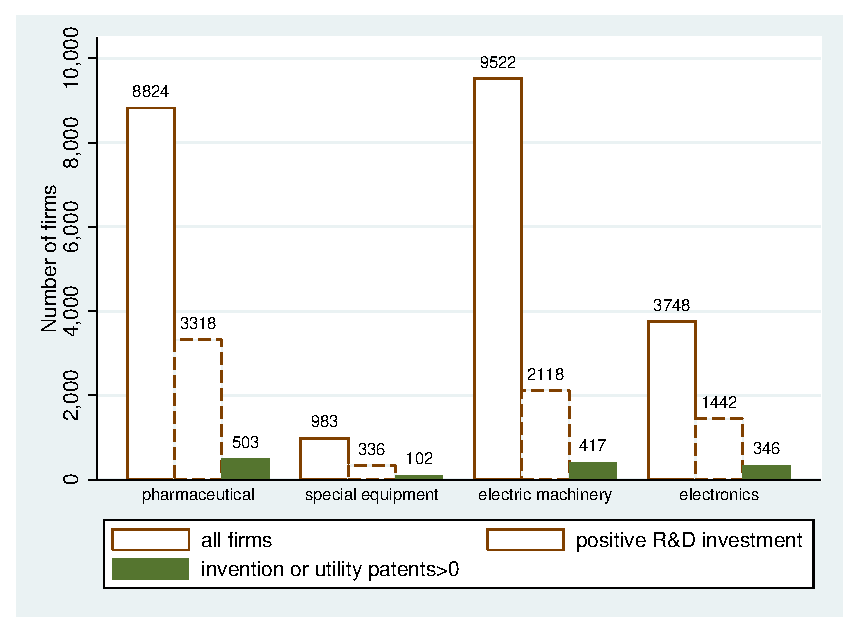
\includegraphics[width=0.8\textwidth]{FirmsCount.eps}
\par\end{centering}

{\small{}Note: numbers are from the final database}{\small \par}
\end{figure}

\par\end{center}

\begin{table}[H]
\centering
\caption{Estimates of demand elasticities}
\label{T11}
\begin{tabular}{lllll}
\toprule 
industry & pharmaceutical & equipment & electronics & machinery \\
\midrule 
$\hat{\sigma}$ &  5.926 & 5.043 & 6.341 & 5.415 \\

$\frac{\hat{\sigma}}{\hat{\sigma}-1}$ & 1.203  & 1.247  & 1.187  & 1.227 \\

\bottomrule 
\end{tabular}
\end{table}

\begin{table}[H]
\centering
\caption{Estimates of productivity evolution equation and cost function}
\label{T12}
\def\sym#1{\ifmmode^{#1}\else\(^{#1}\)\fi}
\begin{tabular}{lllll}
\toprule 
 & \multicolumn{2}{c}{cubic parameterization}\\
\midrule
\multicolumn{5}{l}{\textit{Productivity evolution:}}\\
$rd_t$                    & .00435\sym{**}  & (2.90) \\
$n_{t+1} \times rd_t$     &  .0145\sym{**} & (2.90) \\
$b_{t+1} \times rd_t $     & .0137\sym{*} & (2.76) \\
$\phi_{t}$             & .824\sym{**}  & (14.96)  \\
$\phi_{t}^{2}$         & .503\sym{**} & (2.69)  \\
$\phi_{t}^{3}$         & -1.135\sym{**}& (-14.26)\\
\midrule 
$\rho_{0}$:               &  &  &  & \\
common part               &.0295\sym{**} & (8.34) \\
Pharmaceutical            & -.0144\sym{*}&(-3.90) \\
Electronics               & -.0132\sym{**} &(-3.61)\\
Electric Machinery       & -.0116\sym{**} &(-2.92) \\ 
$\sigma_{\varepsilon}$ & \multicolumn{2}{c}{.10} \\
\midrule 
\multicolumn{5}{l}{\textit{Cost function:}} \\
$k$                      & -.0299\sym{**}& (-25.82)   \\       
$a\in\left(10,\,19\right)$  & .0740\sym{**} &(12.62)\\
$a\in\left(20,\,49\right)$  & 0.111\sym{**}&(12.88)   \\
$a\geq50$                &.149\sym{**}  & (7.84) \\
\midrule              
sample size & \multicolumn{4}{c}{22492}\tabularnewline
\bottomrule
\end{tabular}


\caption*{\small{}Note: T statistics are in parentheses; {*} p$<$0.05, {*}{*}
p$<$0.01. }{\small \par}
\end{table}

\begin{table}[H]
\centering
\caption{Distribution of patent applications conditional on R\&D decision}
\label{T10}
\begin{tabular}{lllll}
\hline\hline
Industries     & $p(0,0)$& $p(1,0)$& $p(0,1)$ & $p(1,1)$ \\
\hline\hline
pharmaceutical & 0.903 & 0.085 & 0.007 & 0.005  \\
equipment      & 0.826 & 0.012 & 0.115 & 0.047 \\
electronics    & 0.899 & 0.009 & 0.069 & 0.023 \\
machinery      & 0.857 & 0.015 & 0.094 & 0.035 \\
\hline\hline 
\multicolumn{5}{l}{\footnotesize Note: $p(x,y)=Prob(n_{t+1}=x, b_{t+1}=y|d_{t}=1)$.}
\end{tabular}
\end{table}

\begin{table}[H]
\centering
\caption{Estimation results of R\&D costs}
\label{T13}
\begin{tabular}{lllll}
\hline\hline
\multicolumn{5}{l}{{\it Panel A }: Estimates for the costs parameters} \\
Sectors & Pharmaceutical & Equipment & Electronics & Machinery \\
\hline
$\kappa^{s}$      & .8981   & 1.7503  & 2.7031   & 1.1807   \\
            & (.0351)   & (.2928)  & (.1249)  & (.0792)  \\
$\kappa ^{m}$     & .1142   & .1080  & .1727   & .1063   \\
            & (.0013)   & (.0040)  & (.0027)   & (.0018)   \\
\hline
LLF         & -4298.48 & -360.44 & -3354.62 & -1611.94 \\
sample size & 8603     & 939     & 9308     & 3604   \\ 
\hline
\multicolumn{5}{l}{{\it Panel B }:Average R\&D costs} \\
Start-up cost                         &0.797 & 1.450 & 2.241 & 0.966 \\
Maintenance cost                       &0.101 & 0.089 & 0.143 & 0.087\\
\hline\hline 
\end{tabular}
\caption*{\small{}Note: Standad errors in the parenthesis are obtained by bootstrapping 100 times. Money units are in million US dollars.}{\small \par}
\end{table}


\begin{table}[H] %short--run benefits of R&D
\centering
\caption{Short-run and long-run benefits of R\&D investment}
\label{T17A}
\begin{tabular}{llllll}
\hline\hline
sectors            & Pharmaceutical & Equipment & Electronics & Machinery&average \\
\hline
I.SHORT RUN: &&&& \\
percentage change & 0.0287 & 0.0300 & 0.0330 & 0.0302 & 0.031 \\
\hline
II.LONG RUN: &&&& \\
percentage change (pp) &&&& \\
mean&0.382  & 0.464  & 0.508  & 0.470  & 0.452 \\
median&0.378  & 0.477  & 0.492  & 0.478  &       \\
std& 0.133  & 0.122  & 0.193  & 0.146  &       \\
absolute change &&&& \\
mean &0.200  & 0.201  & 0.287  & 0.191  & 0.235 \\
median &0.185  & 0.190  & 0.252  & 0.178  &       \\
std& 0.098  & 0.086  & 0.170  & 0.088  & \\     
\hline\hline
\end{tabular}
\caption*{\small{}Note: the absolute change is measured in million USD; the average is a weighted average using the sample size.}{\small \par}
\end{table}


\begin{table}[H] %decomposing the long--run benefits of R&D
\centering
\caption{Decomposition of the Long-run benefits of R\&D investment}
\label{T17C}
\begin{tabular}{lcccc}
\hline\hline
              &Pharmeceutical & Equipment & Electronics & Machinery\\
\hline
\multicolumn{5}{l}{proportional change:}                      \\
no patent  & 0.329 & 0.376 & 0.437 & 0.384 \\
invention  & 0.852 & 0.788 & 1.027 & 0.882 \\
utility    & 0.823 & 0.765 & 0.994 & 0.854 \\
both       & 1.368 & 1.191 & 1.609 & 1.369 \\
total      & 0.382 & 0.464 & 0.508 & 0.470  \\
\hline
\multicolumn{5}{l}{absolute change:}                          \\
no patent  & 0.173 & 0.164 & 0.249 & 0.157 \\
invention  & 0.443 & 0.339 & 0.571 & 0.356 \\
utility    & 0.428 & 0.329 & 0.553 & 0.345 \\
both       & 0.709 & 0.509 & 0.889 & 0.551 \\
total      & 0.200 & 0.201 & 0.287 & 0.191 \\
\hline\hline
\end{tabular}
\caption*{\small{}Note: the absolute change is measured in million USD.}{\small \par}
\end{table}



\begin{table}[H] %decomposing the long--run benefits of R&D
\centering
\caption{Decomposition of the Long-run benefits of R\&D investment: relative importance}
\label{T17D}
\begin{tabular}{lcccc}
\hline\hline
              &Pharmaceutical & Equipment & Electronics & Machinery\\
\hline
no patent  & 0.777 & 0.669 & 0.774 & 0.699 \\
invention  & 0.190 & 0.020 & 0.018 & 0.028 \\
utility    & 0.015 & 0.190 & 0.135 & 0.171 \\
both       & 0.018 & 0.121 & 0.073 & 0.102 \\
\hline\hline
\end{tabular}
\caption*{\small{}Note: the relative importance are measured in 100 percent.}{\small \par}
\end{table}

\begin{table}[H]
\centering
\caption{Estimates of the value of patents}
\label{T18}
\begin{tabular}{lllcllc}
\hline\hline
                     &\multicolumn{3}{c}{invention} &\multicolumn{3}{c}{utility} \\
                        & mean  & median & std   & mean            & median & std   \\
\hline
\multicolumn{7}{l}{proportional change:} \\
Pharmaceutical & 0.547 & 0.552 & 0.180 & 0.674 & 0.681 & 0.219 \\
Equipment      & 0.683 & 0.721 & 0.155 & 0.505 & 0.534 & 0.116 \\
Electronics    & 0.963 & 0.974 & 0.304 & 0.701 & 0.709 & 0.223 \\
Machinery      & 0.788 & 0.823 & 0.216 & 0.598 & 0.625 & 0.166 \\
average        & 0.764 &       &       & 0.666 &       &       \\
\hline
\multicolumn{7}{l}{absolute change:} \\
Pharmaceutical & 0.283 & 0.266 & 0.126 & 0.349 & 0.328 & 0.154 \\
Equipment      & 0.291 & 0.285 & 0.101 & 0.215 & 0.210 & 0.075 \\
Electronics    & 0.529 & 0.483 & 0.251 & 0.385 & 0.351 & 0.184 \\
Machinery      & 0.317 & 0.306 & 0.128 & 0.241 & 0.232 & 0.098 \\
average        & 0.391 &       &       & 0.341 &       &       \\
\hline\hline
\end{tabular}
\caption*{\small{}Note: value of invention (utility) patents is only reported for observations with invention (utility) patents; the absolute change is measured in million USD.}{\small \par}
\end{table}



\begin{center}
\begin{figure}[H]
\caption{Correlation between patent value and knowledge breadth-based patent quality measure}
\label{F5}
\begin{centering}
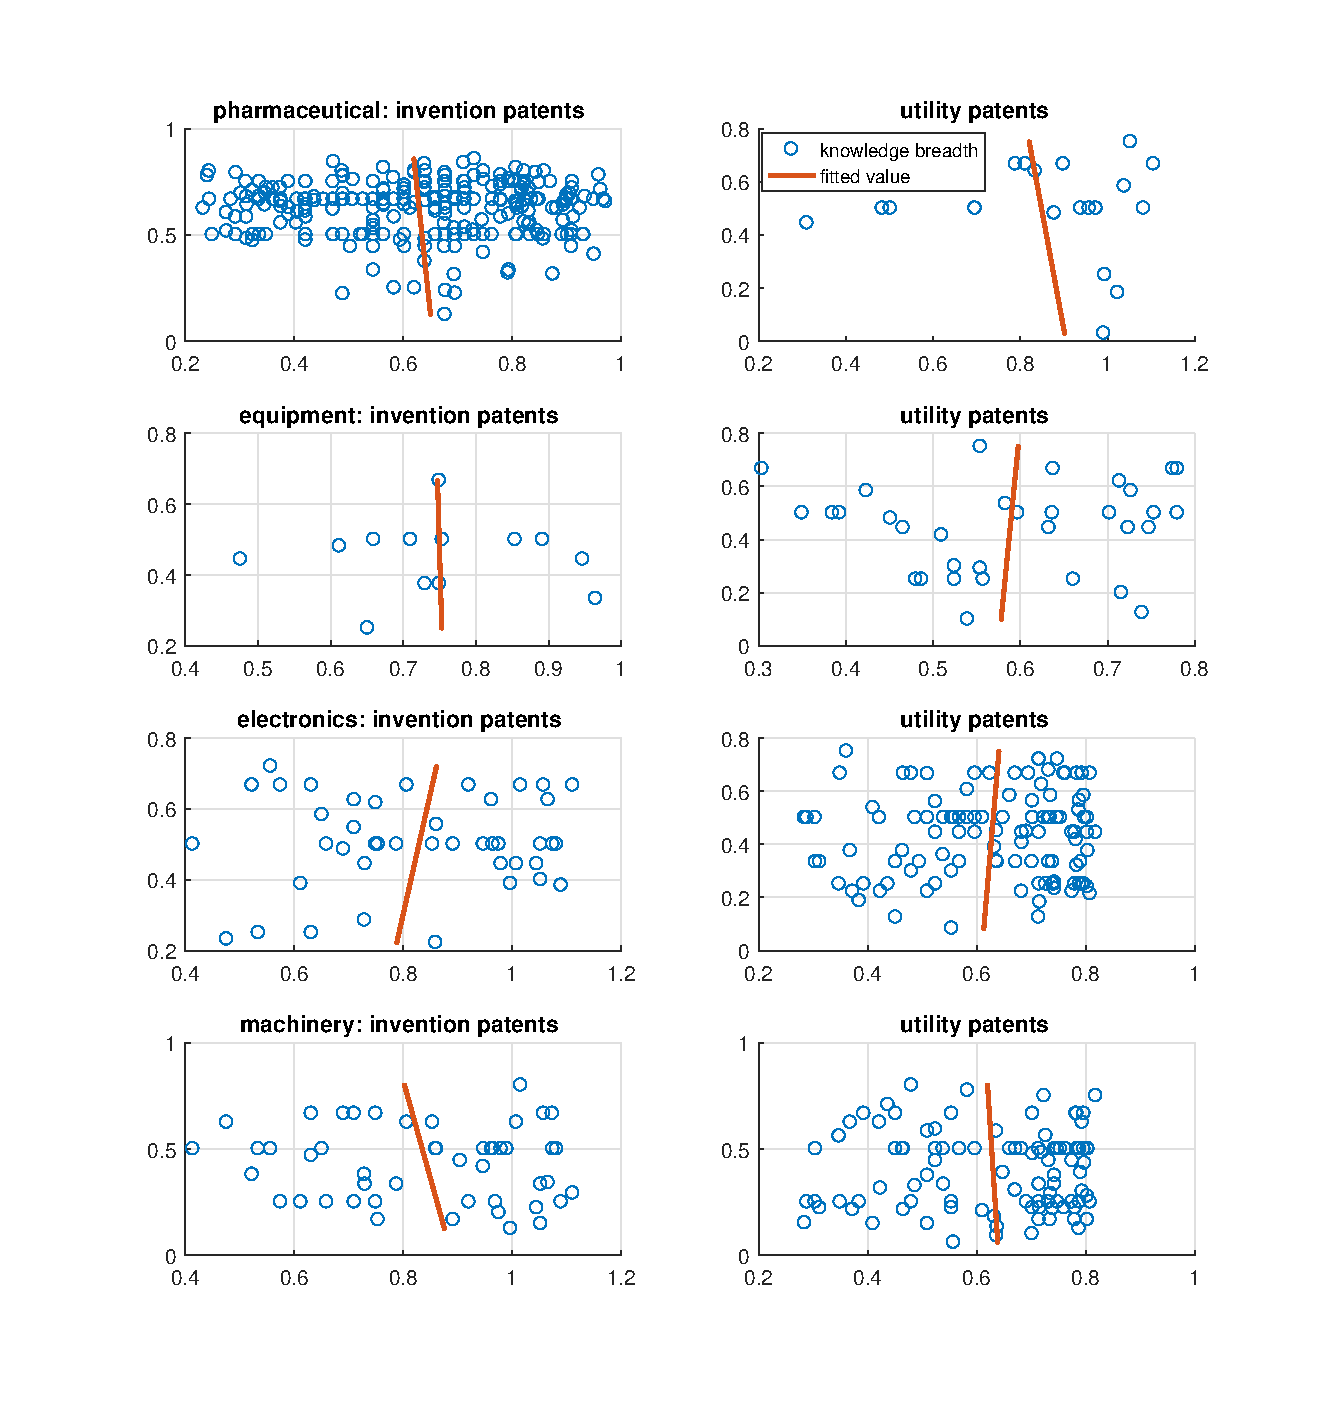
\includegraphics[width=0.9\textwidth]{patcorr.eps}
\par\end{centering}
\caption*{\small{}Note: quality measure is based on \citet{Dang2015}. In all graphs, the horizontal axis is the patent quality measure based on the knowledge width of the patent claim, the vertical axis is the model-generated patent value.}{\small \par}
\end{figure}
\par\end{center}

\begin{center}
\begin{figure}[H]
\caption{Change in firm value caused by different subsidy policies: $\delta^m=0.80$}
\label{F6}
\begin{centering}
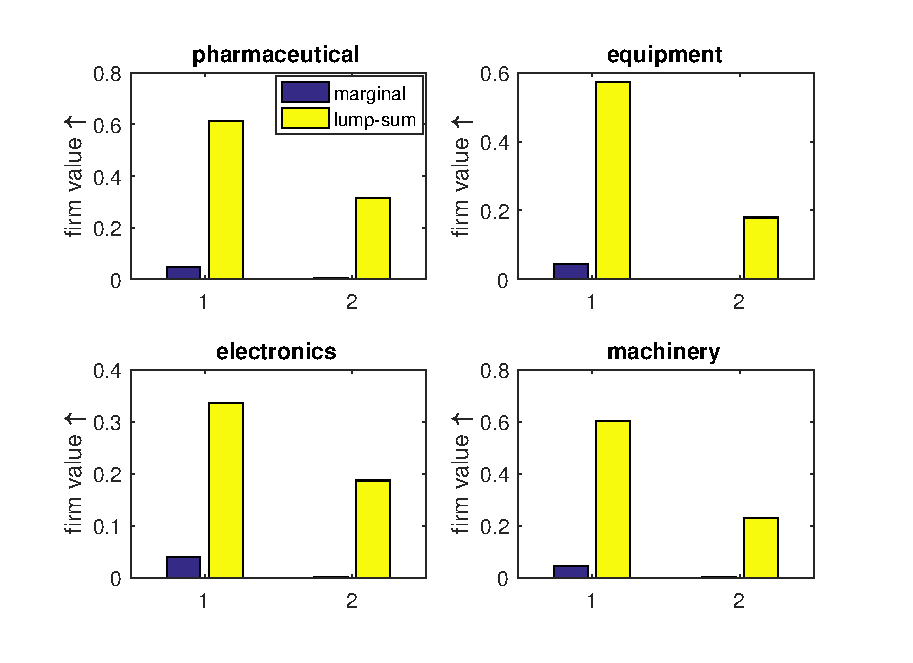
\includegraphics[width=1\textwidth]{FirmvalueChange.eps}
\par\end{centering}
\caption*{\small{}Note: in all the graphs, '1' represents subsidy on the maintenance costs, '2' represents subsidy on the start-up costs. Firm value is measured in 10,000 US dollars.}{\small \par}
\end{figure}
\par\end{center}

\begin{center}
\begin{figure}[H]
\caption{Change in innovation probability caused by different subsidy policies: $\delta^m=0.80$}
\label{F7}
\begin{centering}
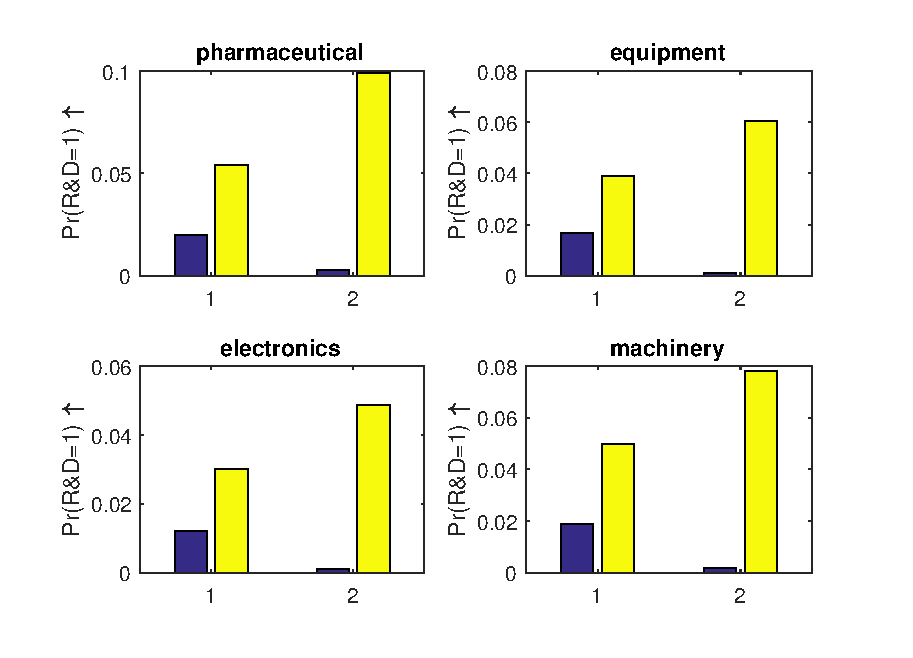
\includegraphics[width=1\textwidth]{ProbChange.eps}
\par\end{centering}
\caption*{\small{}Note: in all the graphs, '1' represents subsidy on the maintenance costs, '2' represents subsidy on the start-up costs.}{\small \par}
\end{figure}
\par\end{center}

\begin{center}
\begin{figure}[H]
\caption{Increase in firm value caused by one unit increase in subsidy: $\delta^m=0.80$}
\label{F8}
\begin{centering}
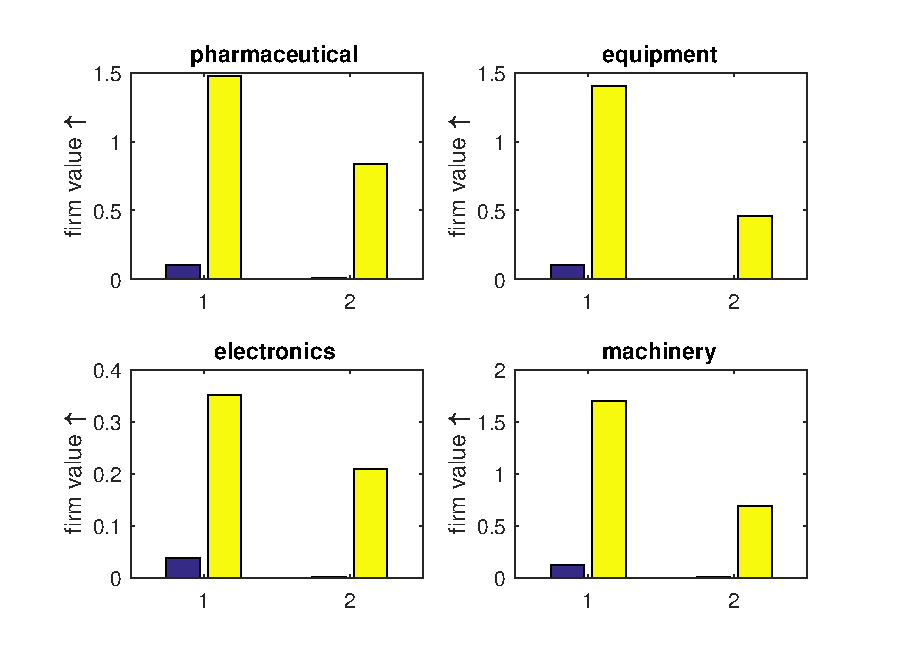
\includegraphics[width=1\textwidth]{valuechangePerUnit.eps}
\par\end{centering}
\caption*{\small{}Note: in all the graphs, '1' represents subsidy on the maintenance costs, '2' represents subsidy on the start-up costs. Firm value is measured in 10,000 US dollars.}{\small \par}
\end{figure}
\par\end{center}

\begin{center}
\begin{figure}[H]
\caption{Increase in innovation probability caused by one unit increase in subsidy: $\delta^m=0.80$}
\label{F9}
\begin{centering}
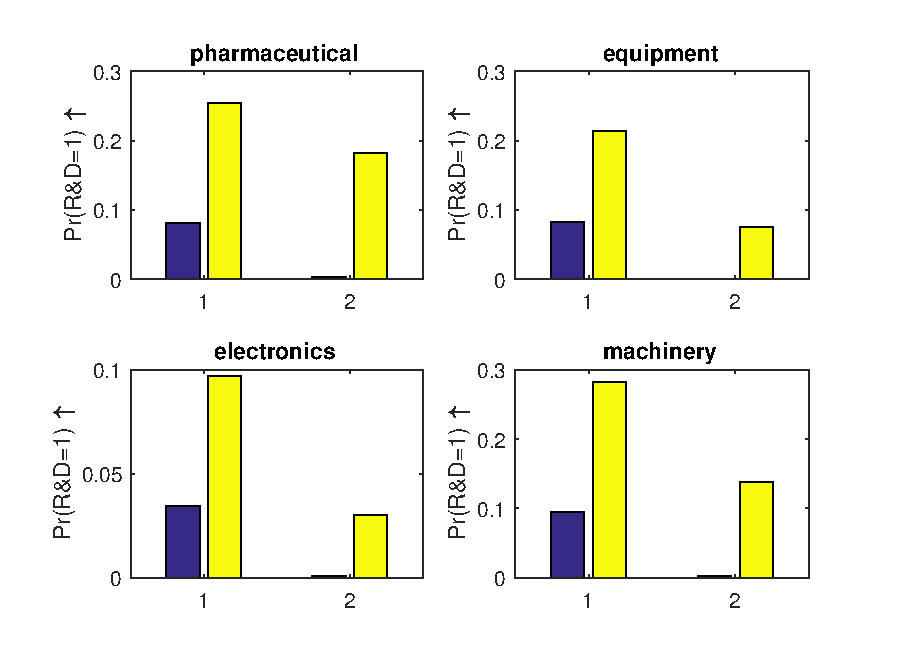
\includegraphics[width=1\textwidth]{probchangePerUnit.eps}
\par\end{centering}
\caption*{\small{}Note: in all the graphs, '1' represents subsidy on the maintenance costs, '2' represents subsidy on the start-up costs. Firm value is measured in 10,000 US dollars.}{\small \par}
\end{figure}
\par\end{center}




\newpage
\setcounter{section}{0}
\renewcommand*{\thesection}{\Alph{section}}
\section*{Appendix (Not for Publication)}
\setcounter{equation}{0}
\numberwithin{equation}{section}
\section{Math}
The firm's profits maximization problem is
\begin{align*}
\max_{L_{it},\,M_{it}} & \left\{ P_{it}Q_{it}-P_{Lt}L_{it}-P_{Mt}M_{it}\right\} \\
s.t.\, & Q_{it}=P_{it}^{-\sigma}P_{t}^{\sigma}Q_{t}\\
 & Q_{it}=\Phi_{it}K_{it}^{\beta_{k}}L_{it}^{\beta_{l}}M_{it}^{\beta_{m}}\exp\left(\beta_{a}a_{it}\right)
\end{align*}
Write the revenue as a function of the output, the first-order conditions
are:
\begin{align}
\left(1-\frac{1}{\sigma}\right)\left(P_{t}^{\sigma}Q_{t}\right)^{\frac{1}{\sigma}}Q_{it}^{-\frac{1}{\sigma}}\frac{\partial Q_{it}}{\partial L_{it}} & =P_{Lt}\\
\left(1-\frac{1}{\sigma}\right)\left(P_{t}^{\sigma}Q_{t}\right)^{\frac{1}{\sigma}}Q_{it}^{-\frac{1}{\sigma}}\frac{\partial Q_{it}}{\partial M_{it}} & =P_{Mt}
\end{align}
where $\frac{\partial Q_{it}}{\partial M_{it}}=\beta_{m}\frac{Q_{it}}{M_{it}}$
and $\frac{\partial Q_{it}}{\partial L_{it}}=\beta_{l}\frac{Q_{it}}{L_{it}}$.
This implies that 
\begin{equation}
M_{it}=\frac{P_{Lt}}{P_{Mt}}\frac{\beta_{m}}{\beta_{l}}L_{it}
\end{equation}
Plugging this back to the foc for $L_{it}$, we obtain
\begin{align}
P_{Lt} & =\beta_{l}\left(1-\frac{1}{\sigma}\right)\left(P_{t}^{\sigma}Q_{t}\right)^{\frac{1}{\sigma}}\frac{Q_{it}^{1-\frac{1}{\sigma}}}{L_{it}}\nonumber \\
 & =\beta_{l}\left(1-\frac{1}{\sigma}\right)\left(P_{t}^{\sigma}Q_{t}\right)^{\frac{1}{\sigma}}\left(\frac{P_{Lt}}{P_{Mt}}\frac{\beta_{m}}{\beta_{l}}\right)^{\frac{\beta_{m}\left(\sigma-1\right)}{\sigma}}\left(\Phi_{it}K_{it}^{\beta_{k}}\exp\left(\beta_{a}a_{it}\right)\right)^{1-\frac{1}{\sigma}}L_{it}^{\frac{\left(\beta_{l}+\beta_{m}\right)\left(\sigma-1\right)}{\sigma}-1}\nonumber \\
\Rightarrow\:L_{it} & =\left[\frac{P_{Lt}\left(\frac{P_{Lt}}{P_{Mt}}\frac{\beta_{m}}{\beta_{l}}\right)^{\frac{\beta_{m}\left(1-\sigma\right)}{\sigma}}}{\beta_{l}\left(1-\frac{1}{\sigma}\right)\left(P_{t}^{\sigma}Q_{t}\right)^{\frac{1}{\sigma}}}\left(\Phi_{it}K_{it}^{\beta_{k}}\exp\left(\beta_{a}a_{it}\right)\right)^{\frac{1-\sigma}{\sigma}}\right]^{\frac{\sigma}{\left(\beta_{l}+\beta_{m}\right)\left(\sigma-1\right)-\sigma}}
\end{align}
Also note that the foc for $L_{it}$ also implies that the revenue
can be expressed as
\begin{equation}
R_{it}=\frac{\sigma P_{Lt}L_{it}}{\beta_{l}\left(\sigma-1\right)}
\end{equation}
 When $\beta_{l}+\beta_{m}=1$, combining these two expressions and
take logs yields:
\begin{equation}
r_{it}=\mu_{0}+\mu_{t}+\left(\sigma-1\right)\left(\beta_{k}k_{it}+\beta_{a}a_{it}+\phi_{it}\right)
\end{equation}
where $\theta=\frac{\sigma}{\sigma-1}$ is the markup and 
\begin{align}
\mu_{0} & =\left(\sigma-1\right)\ln\left(\frac{\sigma-1}{\sigma}\beta_{l}^{\beta_{l}}\beta_{m}^{\beta_{m}}\right)\\
\mu_{t} & =\left(1-\sigma\right)\ln\left(P_{Lt}^{\beta_{l}}P_{Mt}^{\beta_{m}}\right)+\ln\left(P_{t}^{\sigma}Q_{t}\right)
\end{align}
\section{Other Expressions}
\setcounter{equation}{0}
\numberwithin{equation}{section}
\subsection{Decomposition of the R\&D benefits} \label{appa1}
According to our definition, the full expressions of $SB_{xy}$ and $DLB_{lxy}$ are:
\begin{align} \label{bsxy}
SB_{sxy} =&-(1+\theta)\left(\sum_n \sum_b(\rho_4+\rho_5x+\rho_6y)G(n'=x,b'=y|d=1)\right) \\
DLB_{xy} =& \ln \left[ \mathbf{E}V(\phi',d,\mathbf{S}'|\phi,d=1,n'=x,b'=y)\right]-\ln\left[\mathbf{E}V(\phi',d,\mathbf{S}'|\phi,d=0)\right]
\end{align}
where $ \mathbf{E}V(\phi',d,\mathbf{S}'|\phi,d=1,n'=x,b'=y)$ can be computed as
\begin{equation}
\mathbf{E}V(\phi',d,\mathbf{S}'|\phi,d=1,n'=x,b'=y)=\int_{\phi'}V(\phi',d=1,\mathbf{S}')dF(\phi'|\phi,d=1,n=x,b=y)
\end{equation}


\subsection{Equations in the counterfactual analysis}
Using the CDF of exponential distribution and calculate the integral of the RHS of Equations (\ref{wz}) and (\ref{wzf}), we can obtain following expressions:
\begin{align}
W_\tau(\phi, d_{-1}, \mathbf{S})=&\Pi(\phi,\mathbf{S})+\beta \gamma_{\tau}\left[\exp\left(-\frac{\mathbf{E}V_1-\mathbf{E}V_0}{\gamma_{\tau}}\right)-1\right]+\beta \mathbf{E}V(\phi',d,\mathbf{S}'|\phi,d=1) \\
W_\tau^F(\phi, d_{-1}, \mathbf{S})=&\Pi(\phi,\mathbf{S})+\beta \gamma\left[\exp\left(-\frac{\mathbf{E}V_1-\mathbf{E}V_0}{\gamma}\right)-1\right]+\beta\left[\mathbf{E}V(\phi',d,\mathbf{S}'|\phi,d=1)+F_\tau\right] \\
\end{align}

For a firm in state $(\phi, d_{-1}, \mathbf{S})$, its probability of innovating is given by $G_\tau(\Delta EV(\phi, d_{-1}, \mathbf{S}))$ ($G(\Delta EV(\phi, d_{-1}, \mathbf{S}+F_\tau)$) in the regime of proportional (lump-sum) subsidy. Under the assumption that the distribution of $\phi, d_{-1}, \mathbf{S}$ is i.i.d, the increase in the probability of innovation in the industry is given by 
\begin{align}
P_\tau=&\frac{1}{NT}\sum_{i}\sum_{z}\left[G_\tau(\Delta EV(\phi, d_{-1}, \mathbf{S}))-G(\Delta EV(\phi, d_{-1}, \mathbf{S}))\right]\\
P_{\tau}^F=&\frac{1}{NT}\sum_{i}\sum_{z}\left[G(\Delta EV(\phi, d_{-1}, \mathbf{S})+F_\tau))-G(\Delta EV(\phi, d_{-1}, \mathbf{S}))\right]
\end{align}
where $\Delta EV(\phi, d_{-1}, \mathbf{S})=\mathbf{E}V_1-\mathbf{E}V_0$.
Accordingly, we define the probability gains from a unit of subsidy as:
\begin{align}
\chi p_{\tau}=&\frac{1}{NT}\sum_{i}\sum_{z}\frac{\left[G_\tau(\Delta EV(\phi, d_{-1}, \mathbf{S}))-G(\Delta EV(\phi, d_{-1}, \mathbf{S}))\right]G_\tau(\Delta EV(\phi, d_{-1}, \mathbf{S})}{(1-\delta^m)\kappa^mk} \\
\chi p_{\tau}^F=&\frac{1}{NT}\sum_{i}\sum_{z}\frac{\left[G(\Delta EV(\phi, d_{-1}, \mathbf{S})+F_\tau)-G(\Delta EV(\phi, d_{-1}, \mathbf{S}))\right]G(\Delta EV(\phi, d_{-1}, \mathbf{S})+F_\tau)}{(1-\delta^m)\kappa^m k}
\end{align}

\section{Supplementary Empirical Results}

\setcounter{table}{0} %reset the table counter
\renewcommand{\tablename}{Table} % Set the tablename to Panel, instead of Table
\renewcommand\thetable{\thesection.\arabic{table}}
\setcounter{figure}{0}
\counterwithin{figure}{section}
\subsection{More data features}
In this appendix, I present more features of the
data for Chinese high-tech manufacturing firms. In particular, I will discuss the distributional characteristics for patents and the R&D-patents relation. These discussions suggest that the extensive margins of R\&D and patents captures most part of the innovation activities. 

\paragraph{Distribution of patents}

Table \ref{T3} reports the distribution of patents. We can see that
the distribution of patents is highly concentrated at zero for all
three types of patents. The share of firm observations
with zero invention (utility) patents in the final sample is 98.01\%
(95.72\%). This implies that only a small fraction of firms file
patent applications. Focusing on the positive part of the distribution,
the percentage of firm observations filing only one invention (utility)
patent is 1.22\% (2.22\%), and that of firm observations filing two
invention (utility) patents is 0.39\% (0.96\%). Moreover, the number
of firm observations submitting no less than three invention (utility)
patents account for 0.37\% (1.10\%) in the sample. Overall,
these observations imply that the variation in the patents outcome
in positive part (extensive margin) is much less significant than
the change from zero to one (i.e. the extensive margin) for invention
and utility patents. In other wods, among firms that have positive
patent applications, most of the firms (over 50\%) have only one patents. Overall, these results suggest that we have to rely on the variation in extensive margin to identify the productivity effects of the patents.

\begin{table}[H]
\centering
\caption{Distribution of patents for high-tech manufacturing firms}
\label{T3}
\begin{tabular}{lccccc}
\hline\hline
Patents counts & 0       & $\geq 1$ & 1      & 2      & $\geq 3$ \\
\hline
Invention&98.01\% & 1.99\% & 1.22\% & 0.39\% & 0.37\% \\
Utility&95.72\% & 4.28\% & 2.22\% & 0.96\% & 1.10\% \\
\hline\hline
\end{tabular}

{\small{}Note:the percentage represents the share of observations in the specified cohort.}{\small \par}
\end{table}

\paragraph{R\&D-patents relation}

The R\&D-patents linkage is an important part in the structural model to be explained in next section. Since I do not have a direct measure for innovation, I rely on the patents to measure the outcome of innovation. Different from the indicators of process and product innovation used in PRVF, I observe the number of invention patents and/or utility patents filed by each firm. To check the validity of using patents as indicators for innovation, I report the correlation between patents and R\&D at both intensive and extensive margins in Table \ref{T4}. I estimate a linear model relating patents applications to R\&D investment controlling for industry, and year fixed effects. I also control for firm size by use R\&D intensity defined as the ratio of R\&D expenditures to firm's sales. 

\begin{table}[H]
\centering
\caption{Correlation between different margins of R\&D and patents}
\label{T4}
\begin{tabular}{cllllll}
\hline\hline
                                         Dependent variables: & \multicolumn{3}{c}{invention patents} & \multicolumn{3}{c}{utility patents} \\
                                          & extensive   & intensive  & both       & extensive  & intensive  & both      \\
                                          \hline 
\multirow{2}{*}{extensive margin of R\&D} & .0402\sym{***}   & -.216     & .0732\sym{***}  & .0444\sym{***}  & .165      & .121\sym{***}  \\
                                          & (.003)     & (.284)    & (.009)    & (.003)    & (.374)    & (.025)   \\
                                          \hline
\multirow{2}{*}{intensive margin of R\&D} & 0.690\sym{***}    & 3.214      & 1.631\sym{***}   & .403\sym{***}   & 3.319      & 1.350\sym{**}   \\
                                          & (.120)     & (2.196)    & (.364)    & (.109)    & (3.060)    & (.442)   \\
 \hline
\multirow{2}{*}{both}                     & .883\sym{***}   & 1.015      & 1.883\sym{***}   & .780\sym{***}  & 2.870      & 2.302\sym{***}  \\
                                          & (.110)     & (2.497)    & (.327)    & (.107)    & (3.109)    & (.476)  \\
\hline\hline
\end{tabular}
\caption*{\small{}Note: all regression contain industry and year fixed effects. Results in columns (1) and (3) are obtained using all the sample; columns (2) and (4) display the results using observations with positive patent applications. Standad errors are in parentheses.\sym{*} \(p<0.05\), \sym{**} \(p<0.01\), \sym{***} \(p<0.001\)} {\small \par}
\end{table}


The matrix of regression coefficients in Table \ref{T4} show that only the correlation between the extensive margin of invention patents and R\&D investment is positive and highly significant. This implies that the variation in patents outcome at the intensive margin is not well explained by the firm's R\&D effort. Because R\&D is the fundamental source of innovation, we will expect that the variation in patents along the intensive margin will not have significant impact on firm's growth. Another important observation from the table is that the intensive margin of R\&D is an important explanatory variable for the extensive margin of patents outcome. However, the correlation coefficient becomes much larger if we consider both margins of R\&D and use R\&D intensity as the indicator for R\&D. This suggests that the change of R\&D from zero to positive has much larger marginal impact in generating patents. In the data, the fraction of firms with zero patent is around 30\%, while the fraction is increased to be 60\% for firms with at least one invention or utility patent. In contrast, the mean value of R\&D for firms with at least one patent is only slightly higher than firms without any patent. This confirms that the variation in R\&D along the extensive margin is the main driver in explaining the patents outcome. 


\subsection{NLLS estimation} \label{appc2}
As a robustness check, we also try to parameterize $h(\cdot)$ as a quadratic function. The estimation results are reported in Table \ref{TA}. In order to use the first-stage estimates to calculate the value function, we need to check the first-order derivative of $h(\phi_{it},d_{it},n_{it+1},b_{it+1})$ with respect to $\phi_{it}$. To ensure that firms have incentive to invest in R\&D and their value functions are bounded, we require this derivative is between 0 and 1. 

\begin{table}[H]

\centering
\caption{Estimates of productivity evolution equation: supplementary results}
\label{TA}
{
\def\sym#1{\ifmmode^{#1}\else\(^{#1}\)\fi}
\begin{tabular}{l*{1}{cc}}
\hline\hline
\multicolumn{3}{c}{productivity evolution equation  }\\
\hline 
$\omega_t$       &       0.826\sym{**}&     (17.13)\\
$\omega_t^2$     &        0.300\sym{**}&     (15.87)\\

$rd_t$    &     0.00505\sym{**}&      (3.35)\\

$rd_t\times n_{t+1}$      &      0.0153\sym{**}&      (3.04)\\
$rd_t \times b_{t+1}$      &     0.0142\sym{*} &      (2.85)\\
$\beta_k$                  & -0.308\sym{**}    &     (-25.71)\\
\hline
\(N\)       &       22492        &            \\
\hline\hline
\end{tabular}
}

\caption*{\small{}Note:T statistics are in parentheses; {*} p$<$0.05, {*}{*}
p$<$0.01. }{\small \par}
\end{table}

\begin{figure}[H]
  \centering
  \caption{First-order derivative of $h(\cdot)$ with respect to $\phi_{it}$}
  \subfloat[Cubic parameterization]{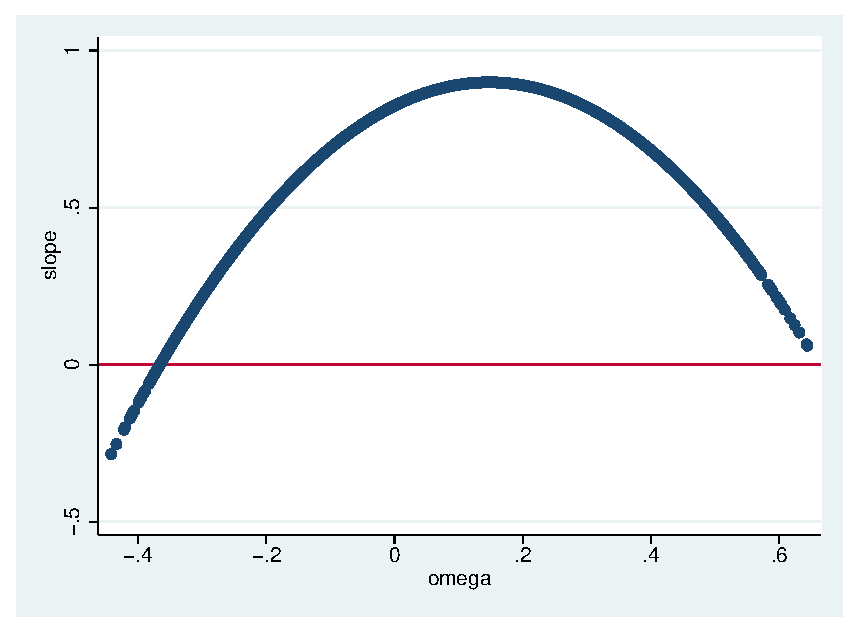
\includegraphics[width=0.45\textwidth]{slope_benchmark.eps}\label{slope1_fig}}
  \hfill
  \subfloat[Quadratic parameterization]{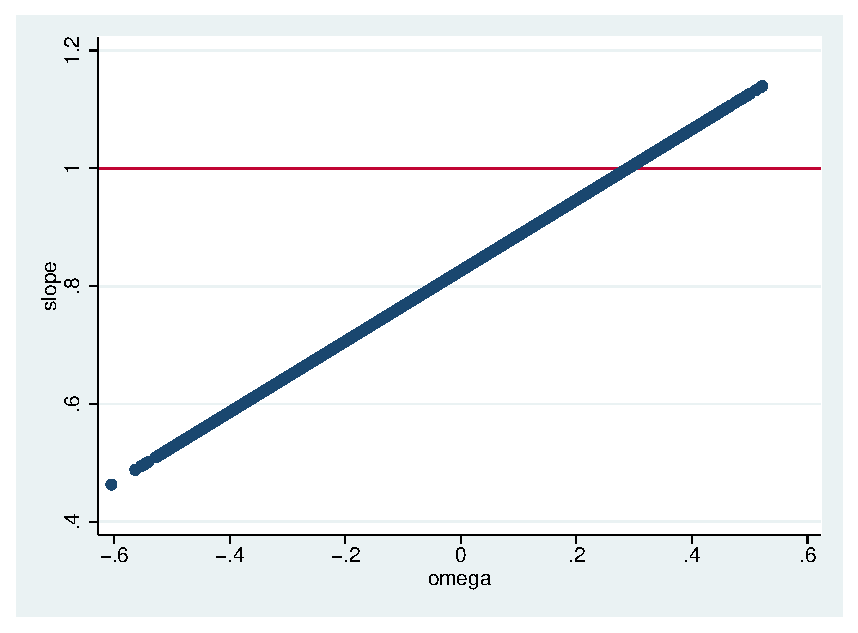
\includegraphics[width=0.45\textwidth]{slope_robustness.eps}\label{slope2_fig}}
 \caption*{Note: in the cubic form, the number of observations that has the slope below zero is 89; in the quadratic equation,the number of observations with slope greater than one is 517. }
\end{figure}

\subsection{Model fitness}
\paragraph{Fitness of predicted revenues} In Figure \ref{F3}, I present a scatter plot to check the relationship between the model predicted revenue and the revenue information in the data. We can see that the predicted revenues concentrates around the 45-degree line, which indicates the revenue equation fits the data well. 

\begin{center}
\begin{figure}[H]
\caption{Model fitness for the revenue data}
\label{F3}
\begin{centering}
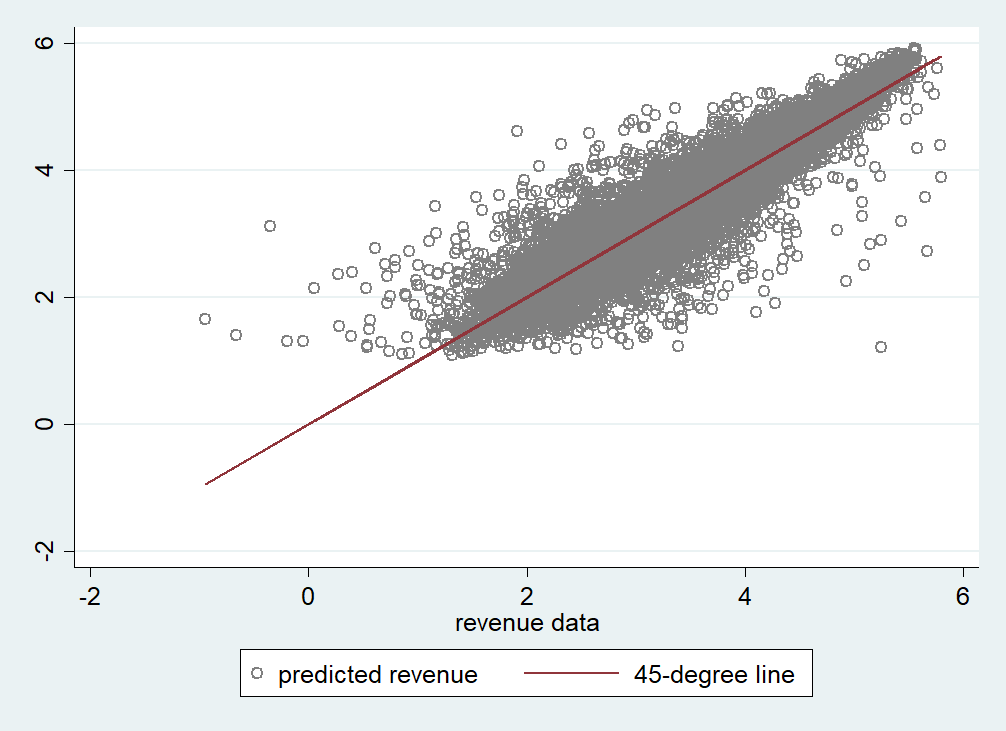
\includegraphics[width=0.8\textwidth]{revenue.png}
\par\end{centering}
\caption*{\small{}Note: sales are in logs of revenues in 100,000 USD.}{\small \par}
\end{figure}
\par\end{center}

\paragraph{Pooled probability of investing in R\&D}
Given current state, we can solve for the probability of undertaking R\&D,$Pr(d=1|\phi,d_{-1},\mathbf{S})$ using equation (\ref{p_d}). Therefore the aggregate hazad function for R\&D choice can be calculated as:
\begin{equation}\label{hazad}
\mathcal{H}=\frac{1}{NT}\sum_{i}^{N}\sum_{t}^{T} Pr(d_{it}=1|\phi_{it},d_{it-1},\mathbf{S}_{it})
\end{equation}
On the other hand, in the data the probability of investing in R\&D is given as
\begin{equation}
\tilde {\mathcal{H}}=\frac{1}{NT}\sum_{i}^{N}\sum_{t}^{T} d_{it}
\end{equation}
I calculate the hazad function for each sector. The results are displayed in Table \ref{T15}. Overall, the estimated model predicts the probability of innovation similar to that exhibited in the data. The model-predicted pooled probability of choosing R\&D is slightly higher, but the difference from the data is around 0.04. Implying that the estimated model captures the innovation decision reasonably well in terms of the probability of choosing innovation for the pooled sample. 

\begin{table}[H]
\centering
\caption{Pooled probability of investing in R\&D}
\label{T15}
\begin{tabular}{lllll}
\hline\hline
Prob. of innovation & Pharmaceutical & Equipment & Electronics & Machinery \\
\hline
model & 0.438 & 0.394 & 0.271 & 0.438 \\
data  & 0.379 & 0.349 & 0.222 & 0.389 \\  
\hline\hline
\end{tabular}
\end{table}

\paragraph{Transition dynamics of R\&D choice}
The transition probability characterizes the dynamics of transition for past R\&D choice to current R\&D decision. Let $d_{-1}\in\{0,1\}$ be the R\&D status in previous year and $d\in\{0,1\}$ be the current R\&D decision, then the transition probabilities are $Q(d|d_{-1})$. I calculate these probabilities in data using a formula as follows:
\begin{equation}
\tilde Q(d=z'|d_{-1}=z)=\frac{\sum_{i}^{N}\sum_{t}^{T} \mathbb{1}\{d_{it}=z',d_{it-1}=z\}}{\sum_{i}^{N}\sum_{t}^{T} \mathbb{1}\{d_{it-1}=z\}}
\end{equation}
where $z,z'\in\{0,1\}$. The model predicts the transition probability for each given state as:
\begin{align}
Q(d=z'|d_{-1}=z)=\frac{1}{NT}\sum_{i}^N\sum_{t}^T Pr(d_{it}=z'|d_{it-1}=z,k_{it})
\end{align}
where $Pr(d_{it}=z'|d_{it-1}=d,k_{it})$ can be obtained using Equation (\ref{p_d}). I calculate these two transition probabilities for each sector and present it in Table \ref{T16}. First, the general patterns of the relative magnitudes of transition probabilities in the data and that predicted by the model are quite similar. In all four industries, the probability of staying in previous state is much higher than transiting to a new state. In other wods, $Q(0,0)$ is larger than $Q(0,1)$, and $Q(1,1)$ is greater than $Q(1,0)$. Second, the probabilities predicted my the estimated model is very close to that observed in the data. These results suggest that the estimated model captures the transition dynamics in the R\&D activities well. 
\begin{table}[H]
\centering
\caption{Transition dynamics of R\&D choice}
\label{T16}
\begin{tabular}{llllll}
\hline\hline
sectors      & source  &$Q(0,0)$  &$Q(0,1)$  &$Q(1,0)$ &$Q(1,1)$ \\
\hline
Pharmeceutical & data  & 0.851 & 0.149 & 0.233 & 0.767 \\
               & model & 0.790 & 0.210 & 0.176 & 0.824 \\
Equipment      & data  & 0.915 & 0.085 & 0.183 & 0.817 \\
               & model & 0.875 & 0.125 & 0.128 & 0.872 \\
Electronics    & data  & 0.930 & 0.070 & 0.257 & 0.743 \\
               & model & 0.885 & 0.115 & 0.194 & 0.806 \\
Machinery      & data  & 0.878 & 0.122 & 0.200 & 0.800 \\
               & model & 0.828 & 0.172 & 0.150 & 0.850 \\
\hline\hline
\end{tabular}
\caption*{\small{}Note: $Q(z',z)=Pr(d=z'|d_{-1}=z)$}{\small \par}
\end{table}

\subsection{Counterfactural analysis}

\paragraph{Full results for all the counterfactual experiments}\label{appc3}
We conduct three experiments in which $\delta^m$ is chosen to be 10\%, 15\%, and 20\%. The full estimation results are reported in Tables \ref{TB}, \ref{TC}, and \ref{TD}. We can observe that these results uniformly show that financing maintenance costs is more effective than financing start-up costs. More importantly, lump-sum subsidy is has larger positive impact on the firm value and the probability of innovation. 

\begin{sidewaystable}
\begin{table}[H]
\caption{Proportional and lump-sum subsidy: $\delta^m=.90$}
\centering
\label{TB}
\begin{tabular}{lllllllll}
\hline\hline
type of subsidy              & \multicolumn{4}{c}{Proportional}                     & \multicolumn{4}{c}{Lump-sum}                         \\\cmidrule{2-9}
sectors                      & pharmaceutical & equipment & electronics & machinery & pharmaceutical & equipment & electronics & machinery \\
\hline 
maintenance costs:           &                &           &             &           &                &           &             &           \\
firm value \uparrow        &0.023 & 0.021 & 0.019 & 0.022 & 0.296 & 0.273 & 0.162 & 0.293 \\
per unit                    & 0.099 & 0.097 & 0.036 & 0.114 & 1.378 & 1.300 & 0.326 & 1.602 \\
innovation Prob. \uparrow   &0.010 & 0.008 & 0.006 & 0.010 & 0.038 & 0.028 & 0.019 & 0.036 \\
per unit                    &0.078 & 0.082 & 0.033 & 0.092 & 0.334 & 0.292 & 0.113 & 0.380 \\
\hline
start-up costs:               &                &           &             &           &                &           &             &           \\
firm value \uparrow      &0.002 & 0.001 & 0.001 & 0.001 & 0.137 & 0.078 & 0.084 & 0.100 \\
per unit                 &0.008 & 0.002 & 0.002 & 0.005 & 0.659 & 0.372 & 0.172 & 0.552 \\
innovation Prob. \uparrow&0.002 & 0.001 & 0.001 & 0.001 & 0.052 & 0.031 & 0.025 & 0.041 \\
per unit                 &0.004 & 0.001 & 0.001 & 0.002 & 0.152 & 0.061 & 0.025 & 0.113 \\ 
\hline\hline
\end{tabular}
\caption*{\small{}Note:units is in 10,000 US dollars.}{\small \par}
\end{table}
\end{sidewaystable}

%  15% reduction
\begin{sidewaystable}
\begin{table}[H]
\caption{Proportional and lump-sum subsidy: $\delta^m=.85$}
\centering
\label{TC}
\begin{tabular}{lllllllll}
\hline\hline
type of subsidy              & \multicolumn{4}{c}{Proportional}                     & \multicolumn{4}{c}{Lump-sum}                         \\\cmidrule{2-9}
sectors                      & pharmaceutical & equipment & electronics & machinery & pharmaceutical & equipment & electronics & machinery \\
\hline 
maintenance costs:           &        &        &        &        &        &        &        &   \\
firm value \uparrow      &0.035 & 0.033 & 0.029 & 0.034 & 0.454 & 0.416 & 0.248 & 0.447 \\
per unit                &0.102 & 0.100 & 0.037 & 0.117 & 1.436 & 1.342 & 0.340 & 1.661 \\
innovation Prob. \uparrow  &0.015 & 0.013 & 0.009 & 0.014 & 0.048 & 0.035 & 0.025 & 0.045 \\
per unit              &0.079 & 0.083 & 0.034 & 0.093 & 0.292 & 0.250 & 0.105 & 0.327 \\
\hline
start-up costs:               &        &        &        &        &        &        &        &        \\
firm value \uparrow        &0.003 & 0.001 & 0.002 & 0.001 & 0.221 & 0.125 & 0.133 & 0.162 \\
per unit            & 0.008 & 0.002 & 0.002 & 0.005 & 0.747 & 0.416 & 0.190 & 0.620 \\
innovation Prob. \uparrow  &0.002 & 0.001 & 0.001 & 0.001 & 0.076 & 0.046 & 0.037 & 0.060 \\
per unit             &0.004 & 0.001 & 0.001 & 0.002 & 0.168 & 0.068 & 0.028 & 0.126 \\
\hline\hline
\end{tabular}
\caption*{\small{}Note:units is in 10,000 US dollars.}{\small \par}
\end{table}
\end{sidewaystable}

\begin{sidewaystable}
\begin{table}[H]
\caption{Proportional and lump-sum subsidy: $\delta^m=.80$}
\centering
\label{TD}
\begin{tabular}{lllllllll}
\hline\hline
type of subsidy              & \multicolumn{4}{c}{Proportional}                     & \multicolumn{4}{c}{Lump-sum}                         \\\cmidrule{2-9}
sectors                      & pharmaceutical & equipment & electronics & machinery & pharmaceutical & equipment & electronics & machinery \\
\hline 
maintenance costs:           &        &        &        &        &        &        &        &        \\
firm value \uparrow   & 0.047 & 0.044 & 0.039 & 0.046 & 0.615 & 0.575 & 0.336 & 0.604 \\
per unit &0.105 & 0.103 & 0.039 & 0.120 & 1.478 & 1.405 & 0.351 & 1.703 \\
innovation Prob. \uparrow &0.020 & 0.017 & 0.012 & 0.019 & 0.054 & 0.039 & 0.030 & 0.050 \\
per unit            &0.081 & 0.083 & 0.035 & 0.094 & 0.254 & 0.215 & 0.097 & 0.282 \\
firm value \uparrow      &0.004 & 0.001 & 0.002 & 0.002 & 0.316 & 0.179 & 0.187 & 0.231 \\
per unit            &0.008 & 0.002 & 0.002 & 0.005 & 0.836 & 0.461 & 0.208 & 0.689 \\
innovation Prob. \uparrow &0.003 & 0.001 & 0.001 & 0.002 & 0.099 & 0.060 & 0.049 & 0.078 \\
per unit            &0.004 & 0.001 & 0.001 & 0.002 & 0.182 & 0.075 & 0.030 & 0.138 \\
\hline\hline
\end{tabular}
\caption*{\small{}Note:units is in 10,000 US dollars.}{\small \par}
\end{table}
\end{sidewaystable}

\end{document}
